\documentclass{l4proj}

\usepackage{alltt}
\usepackage{microtype}
\usepackage{textcomp}
\usepackage[small,bf]{caption}
\usepackage{subcaption}
\usepackage{multirow}
\usepackage{enumitem}
\usepackage{booktabs}

\usepackage[usenames, dvipsnames]{color}
\usepackage{listings}
\lstset{
	basicstyle=\ttfamily
}

\usepackage{graphicx}
\graphicspath{{./images/}}

\usepackage[]{hyperref}
\hypersetup{
    colorlinks = true,
    citecolor = black,
    linkcolor = black,
    urlcolor = black,
}

%%%%%%%%%%%%%%%%%%%%%%%%%%%%%%%%%%%%%%%%%%%%%%%%%%%%%%%%%%%%%%%%%%%%%%%%%%%%%%%%%%%%%%%%%%%%%%%%%%%%

\begin{document}

\title{Visual Control of a Hexapod Robot}
\author{Daniel Callander}
\date{March 28, 2014}
\maketitle

%%%%%%%%%%%%%%%%%%%%%%%%%%%%%%%%%%%%%%%%%%%%%%%%%%%%%%%%%%%%%%%%%%%%%%%%%%%%%%%%%%%%%%%%%%%%%%%%%%%%

\begin{abstract}
Robot control systems require a large underlying infrastructure of software to facilitate any complex behaviour. Typical systems require a means for communicating with hardware, locomotion control for movement, vision systems for guidance and environment mapping, autonomous navigation, means of user interaction, and so on. Each of these components requires a deep understanding of the subject matter and an immense number of person hours to design, implement, and test.

We implement a robot control system for a hexapod-type robot using the Robot Operating System (ROS) as a framework, an open-source framework designed specifically for building robot control systems. Through this implementation, we show that it is possible to endow a robot with these complex behaviours---specifically visual odometry, environment mapping and autonomous navigational functionalities---without the need to invest a large number of person hours. The key advantage of ROS is its vast amount of standard and community-provided packages which implement the necessary functionality for these complex behaviours. We make great use of these packages, offloading the complexities of development to those who are more qualified. 

Furthermore, we show that it is possible to implement these behaviours on a robot built using only consumer components rather than expensive research hardware. An RGB-D camera is used as the primary sensor for understanding the environment, which is used to provide mapping and positional information throughout the control system.
\end{abstract}

\renewcommand{\abstractname}{Acknowledgements}
\begin{abstract}
I would like to thank Dr. Paul Siebert for providing me with his invaluable guidance and expertise throughout the project. It would have been very tough going without his help! 

\noindent
I would also like to thank my fantastic friends and family for their support during the final stages of the project, especially for their proof-reading services for which I am extremely grateful.

\noindent
Finally, it would be rude of me not to thank the robot in some form for remaining (mostly) intact throughout the project. Even though the legs fell off a few times, everything remained working right to the very end.

--- Daniel Callander, 2014
\end{abstract}

\educationalconsent
\tableofcontents

\chapter{Introduction}
\pagenumbering{arabic}

%%%%%%%%%%%%%%%%%%%%%%%%%%%%%%%%%%%%%%%%%%%%%%%%%%%%%%%%%%%%%%%%%%%%%%%%%%%%%%%%%%%%%%%%%%%%%%%%%%%%

The objective of this project was to implement a control system for an existing hexapod-type robot (shown in Figure~\ref{fig:hexapod}) through the use of the Robot Operating System (ROS) \cite{ros_site}. By attempting to implement a number of complex behaviours, such as environment mapping and autonomous navigation, we aimed to evaluate the usefulness of ROS as a framework for rapidly developing these control systems. Specifically, we looked to explore a range of standard and community-provided packages available for use through ROS which provide state-of-the-art functionality, including those that were necessary for this control system.

\begin{figure}[t]
    \centering
    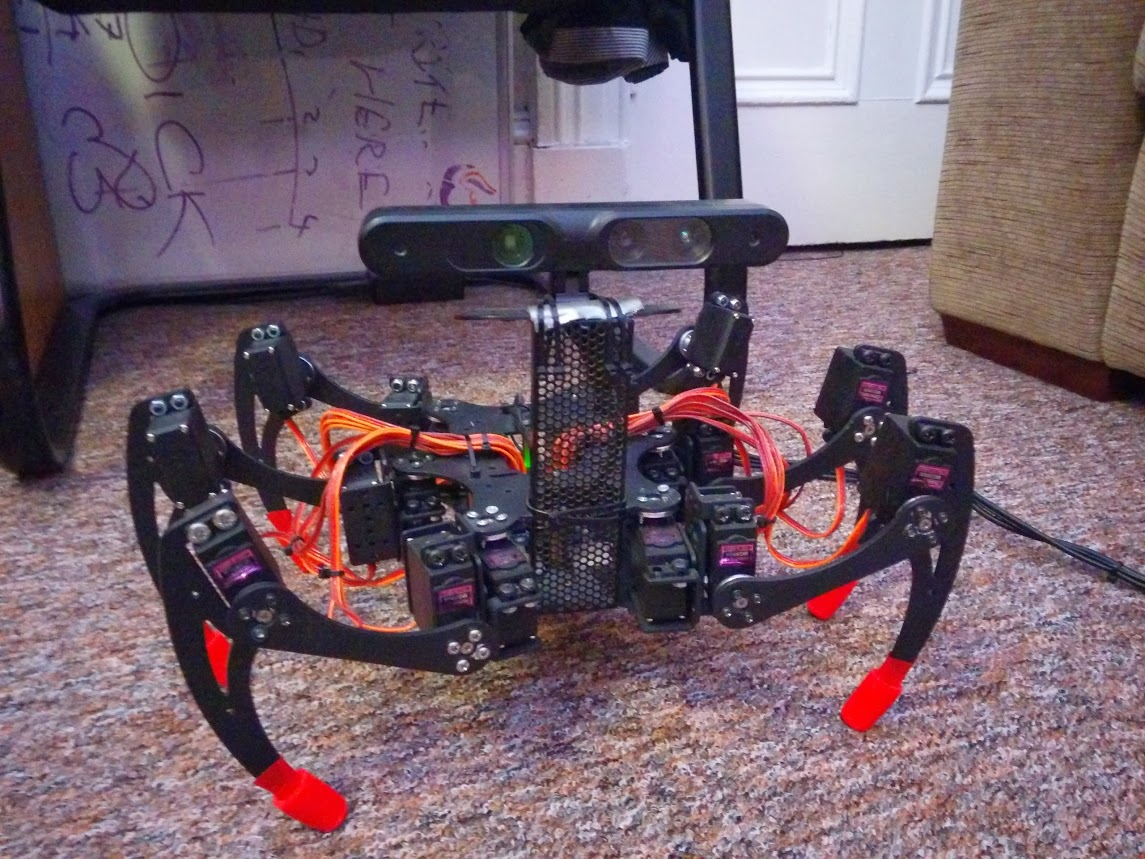
\includegraphics[width=10cm]{hexapod_body1}
    \caption{This hexapod-type which is used as the target hardware platform for this project. The robot has eighteen actuators; three on each limb. A RGB-D camera sits atop as the primary sensor, providing the robot with a 3D view of its immediate environment. A controller sits within the base of the robot, providing the necessary signals to operate the actuators. A bundle of cables protrudes from the back connecting the hardware to a nearby computer for operation, as well as a power source.}
    \label{fig:hexapod}
\end{figure}

This report will detail how this objective was achieved with great success. Through the use of ROS and its packages, it was possible to implement a control system that provides a number of these complex behaviours with relative brevity and simplicity. The resulting robot control system has a number of impressive capabilities:

\begin{description}
	\item[Hardware Interaction] \hfill \\
	The system is capable with interacting with the RGB-D camera and servo controller on-board the robot. Commands can be sent through the system to the controller, allowing for the movement of any particular actuator. Image data from the sensor is received, processed, and then broadcast throughout the system, such that any subsystem needing the imagery can access it.

	\item[Locomotion] \hfill \\
	The system allows the robot to walk with a tripod-type walk gait in an abstracted manner. This abstraction allows any control subsystems to request linear and angular movements, without regard as to the specific actuator commands. The system also provides a means for calibrating the actuators, allowing for movements to be made precisely. Additionally, the robot can be manually controlled via a standard game controller.

	\item[Sensing] \hfill \\
	The system is capable of building a 3D map of the environment around the robot, updating in real-time as the robot moves around. This map is stored in an efficient manner, allowing the system to quickly determine if any obstacles are nearby. Additionally, the system is capable of localising the position of the robot relative to the environment.

	\item[Navigation] \hfill \\
	The system is capable of fully autonomous navigation. Given a target position, the system will determine the most efficient path through the known environment and then supply the appropriate commands to move the robot to that position. Should the robot encounter any new obstacles, the path will be recalculated in real-time to avoid that obstacle.

\end{description}

Without access to the packages available for use through ROS, each of these capabilities would have taken a great number of man hours to develop, test and integrate. 

\section{Motivation}

\section{Overview} 
\chapter{Background}
\label{chap:background}

For any advanced robot to operate correctly, a vast infrastructure of software is generally required. Developing this directly without the use of any frameworks or libraries would require a large amount of person hours, in terms of both design, implementation and integration time. Many different subsystems are required, each of which would require a deep technical understanding of the underlying intricacies. Typical systems require a means for communicating with hardware, locomotion control for movement, vision systems for guidance and environment mapping, autonomous navigation, means of user interaction, and so on. The complexity of each of these is such that they are research fields in their own right. 

However, through the use of ROS it is possible to gain access to these state-of-the-art functionalities free of charge, both in terms of cost and in person hours. The open-source nature of ROS is such that any innovations made by other developers can be easily shared to with the rest of the community. This offloads the complex understanding to smaller development teams which have expertise in that particular area.

The following sections in this chapter elaborate on the features of the ROS and our robot hardware, explaining why they are relevant to this project. A discussion will also be made around the background in general, as well as any existing research. This will provide a basis of understanding necessary for the implementation chapter and beyond.

%%%%%%%%%%%%%%%%%%%%%%%%%%%%%%%%%%%%%%%%%%%%%%%%%%%%%%%%%%%%%%%%%%%%%%%%%%%%%%%%%%%%%%%%%%%%%%%%%%%%

\section{Robot Operating System}

The \emph{Robot Operating System} (ROS) is an open-source framework for creating robot control systems, developed by \emph{Willow Garage} \cite{ros_paper}. ROS can be primarily thought of as a message-passing framework. A number of discrete processes, perhaps some even on a remote machine, communicate through a single broker service (the ROS "master") using an XMLRPC-based API \cite{ros_paper}. Each process performs a small part of a larger task, sharing data with other nodes through common data types.

ROS functions as a distributed system by default. Specifically, the processes can run on a machine different from that of the broker. The processes can then connect to the broker over a network, receiving data seamlessly from any other processes in the system. In cases where nodes are running on the same machine as the broker, they are simply connecting to the local machine. This can be used to offload complex computations onto another machine as necessary. To give an example, an embedded system on a robot running ROS can be collecting sensor data and issues hardware commands. This embedded system can then be communicating to a more powerful machine, acting as a base station. This base station can perform the more complex operations such as sensor data interpretation and path planning, relaying the commands back to the embedded system to be carried out.

\subsection{Supported Platforms}
At the time of writing, the latest version of ROS is \emph{Hydro Medusa} which primarily targets the \emph{Ubuntu} Linux distrubution, specifically versions 12.04 (LTS) to 13.04 \cite{ros_wiki_installation, ros_wiki_installation_ubuntu}. An Ubuntu repository containing binaries for ROS and its standard library of packages is available allowing for a trivial installation process, as well as allowing any updates to be delivered and installed with simplicity.

Experimental support is also available for other Linux distributions and systems, such as Ubuntu ARM, OS X, Debian, Arch Linux, Windows, and a number of embedded platforms \cite{ros_wiki_installation}. As the source code for ROS is freely available, it is possible to compile it on any system as long as the relevant supporting libraries are available.

\subsection{Nodes}
In ROS terminology, a processes is referred to as a \emph{node}. A node is simply a process that is connected to the ROS broker, performing some sort computation \cite{ros_paper}.

Nodes need not be tied to any particular programming language \cite{ros_paper}. Nodes are developed using a particular \emph{client library}, of which many are available. These are libraries developed for a particular language or ecosystem which provide an abstraction layer for interfacing with ROS. The two most used client libraries are \emph{roscpp} and \emph{rospy} which target C++ and Python respectively \cite{ros_wiki_clientlibraries}. There are also a number of experimental client libraries available for other systems such as Java, Android, C\#, and Arduino, among others \cite{ros_wiki_clientlibraries}.

\begin{figure}[!h]
    \centering
    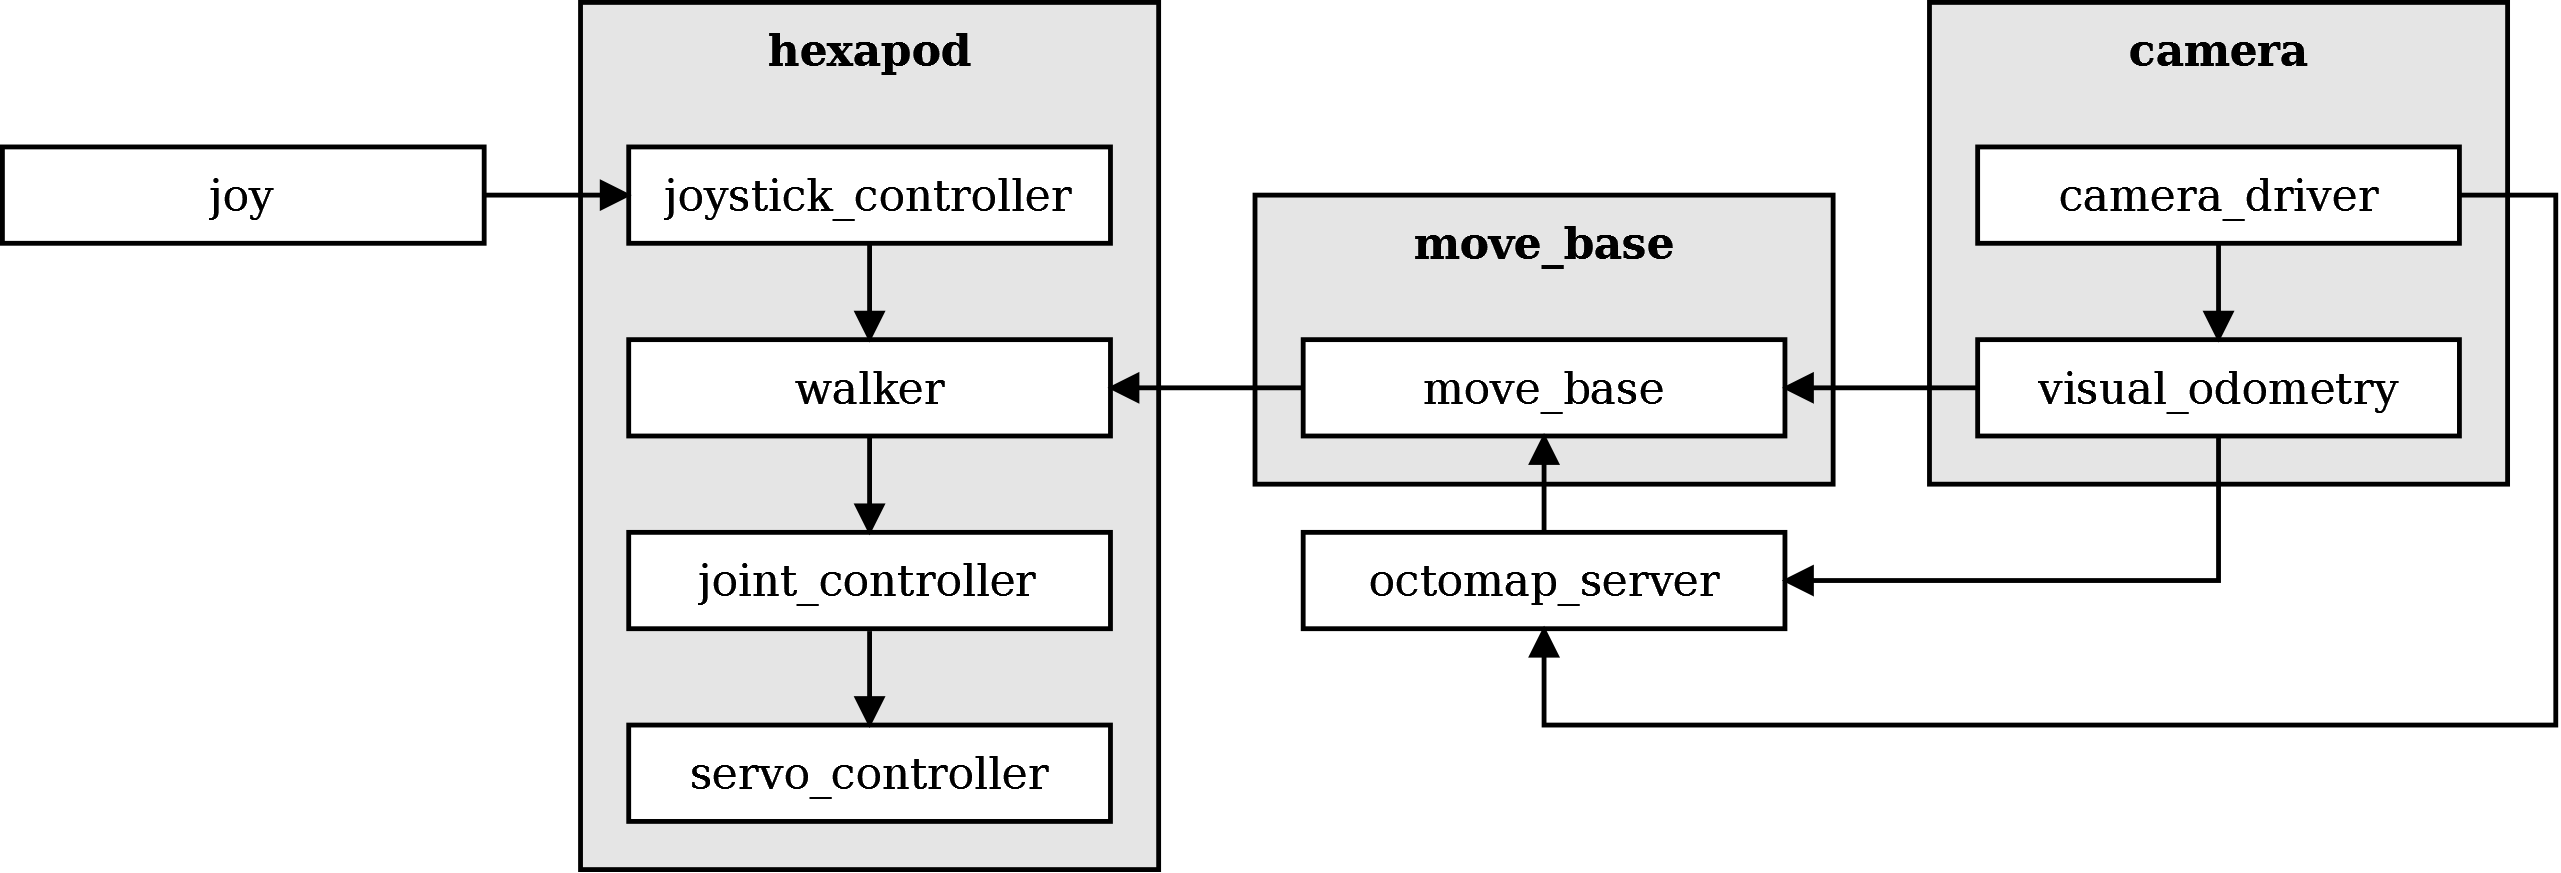
\includegraphics[width=16cm]{nodes.png}
    \caption{A simplified diagram showing an example of node relations, modelled after the implemented robot system. White boxes represent particular nodes, while the grey boxes surrounding them represent a namespace in which they exist. Arrows between nodes indicate a communication flow.}
    \label{fig:nodes}
\end{figure}

As intraprocess communication can be somewhat costly in terms of performance, ROS provides a means for running multiple nodes in the same process via \emph{nodelets} \cite{ros_wiki_nodelet}. This allows messages to be passed in a ``zero-copy'' manner, as pointers to memory locations for any messages can be shared directly. Nodes must be modified to support this behaviour, however, as they must export some class that can be dynamically loaded by a \emph{nodelet manager}. This feature is used extensively when real-time performance is required such as with computer vision related tasks, for example.

\subsection{Topics \& Services}
Node communication is done through \emph{topics} in a one-to-many fashion \cite{ros_paper}. Broadcasting is done asynchronously, such that a broadcasting node can continue operating without regard as to which nodes receive the message. Any other node can then subscribe to that particular topic, receiving messages through a callback for processing. Each topic has a given resource name which is used to uniquely identify that topic.

A topic is defined with a given \emph{message} type through \emph{msg} files. Messages are simple data structures consisting of a number of typed data fields. Each data field has a unique name and can be of a number of built-in primitive types, as well as other arbitrarily nested data structures such as arrays and even other messages. A simple example of this would be the \texttt{Point} message from the \texttt{geometry\_msgs} package. This message consists of three \texttt{float64} fields named \texttt{x}, \texttt{y}, and \texttt{z} \cite{ros_api_point_msg}.

ROS also provides a \emph{request-response} style method of communication through \emph{services} \cite{ros_wiki_services}. In this case, a \emph{service} type is defined in a format similar to topic messages through \emph{srv} files. However, the difference is that two messages are defined in one file---one for the request and the other for the response. This communication method is synchronous in that a requesting node will block until a response is given. 

\subsection{Resource Names}

Each resource in the system has a unique name and can be placed into a particular namespace. This gives each resource a unique \emph{graph resource name} which can be used to identify this resource elsewhere throughout the system. As the name suggests, the layout of a ROS system can be thought of as a graph or tree. Some examples of \emph{graph resource names} are shown in \autoref{tab:graph_resource_names}.

\begin{table}[!h]
    \centering
    \begin{tabular}{  l l  }
        \toprule
        \textbf{Path} & \textbf{Description} \\
        \midrule
        \texttt{/} & the global namespace \\
        \texttt{/hexapod/} & the \texttt{hexapod} namespace \\
        \texttt{/hexapod/servo\_controller} & a \texttt{servo\_controller} node \\
        \bottomrule
    \end{tabular}
    \caption{Some examples of graph resource names.}
    \label{tab:graph_resource_names}
\end{table}

Nodes, topics, and services must all have unique \emph{graph resource names} to identify them within the system. Using namespaces, it is possible to run multiple instances of a particular node such that they do not conflict with each other. Any topics that they would use can also be remapped to point to one that is more appropriate for its usage.

\subsection{Packages}
A collection of nodes providing a particular set of functionalities---e.g., path planning for autonomous navigation---can be grouped and distributed as \emph{packages} \cite{ros_paper}. This can be used to divide nodes in a control system into logical subsystems. By developing nodes and packages in a generic way, they can also act as a means for providing drop-in functionality.

Users are encouraged to share and distribute any developments they make by hosting repositories of their code, preferably on \emph{GitHub} \cite{ros_wiki_getinvolved}. Contributors can then request that their repository be listed on a package index on the ROS website \cite{ros_wiki_getinvolved}. This aspect is a particular advantage of ROS as there is a wide array of packages available for usage. Additionally, as ROS provides a number of common data types used in robotics, packages from different vendors can interact with one another with relative ease.

\subsection{Standard Packages \& Utilities}
The standard ROS distribution contains a number of standard packages and utilities. These provide a number of essential features that streamline the entire development process. A number of these are particularly useful for use with our robot control system.

\subsubsection{roslaunch: Programatically Start Nodes}
While nodes can launched manually, ROS provides a means for large sets of nodes programmatically via \emph{roslaunch} \cite{ros_paper, ros_wiki_roslaunch}. This tool allows developers to specify a set of nodes to be ran, along with a number of parameters, in XML configuration files (``launch files'' in ROS terminology). \emph{roslaunch} provides a number of useful features:

A key feature is the ability to specify which namespace a particular set of nodes is in as mentioned previously. This allows multiple nodes of the same type to be launched without conflict. Any topic used by a node can also be remapped to one more appropriate. This means that nodes can be built generically, assuming that their topics will be remapped to fulfil some specific purpose. An example of this is the \texttt{depthimage\_to\_laserscan} node, which converts a depth image into a format usable by nodes expecting laser scan data. This node expects the depth image to be transmitted on an \texttt{image} topic assuming that this will be remapped to the actual depth image.

Parameters can also be specified in a standard format which the nodes can then read from on launch. This allows any node to be reconfigured as required as long as it provides a means of doing so, making any implemented node much more flexible and general purpose. Without this, nodes would have to result to using some other method of configuration such as domain-specific files or even require their source code to be changed---neither of which would function particularly well in large systems.

Launch files can also include other launch files. Generally, a package will provide a launch configuration that starts all the necessary nodes to provide dealing with this package. This can be used to create a ``master'' configuration that launches a number of subsystems to implement some overall control system.

\subsubsection{rviz: Visualising Sensor Data}

In addition to providing autonomous behaviour, it is often necessary that a control system must be able to provide some useful visualisations to the user operating the system. This can be much more helpful for gaining an understanding of what data the system is receiving versus trawling through text logs alone. Rather than having to develop new visualisation software for every robot system, ROS provides a generic means for achieving this via \emph{rviz} \cite{ros_wiki_rviz}.

\begin{figure}[!h]
    \centering
    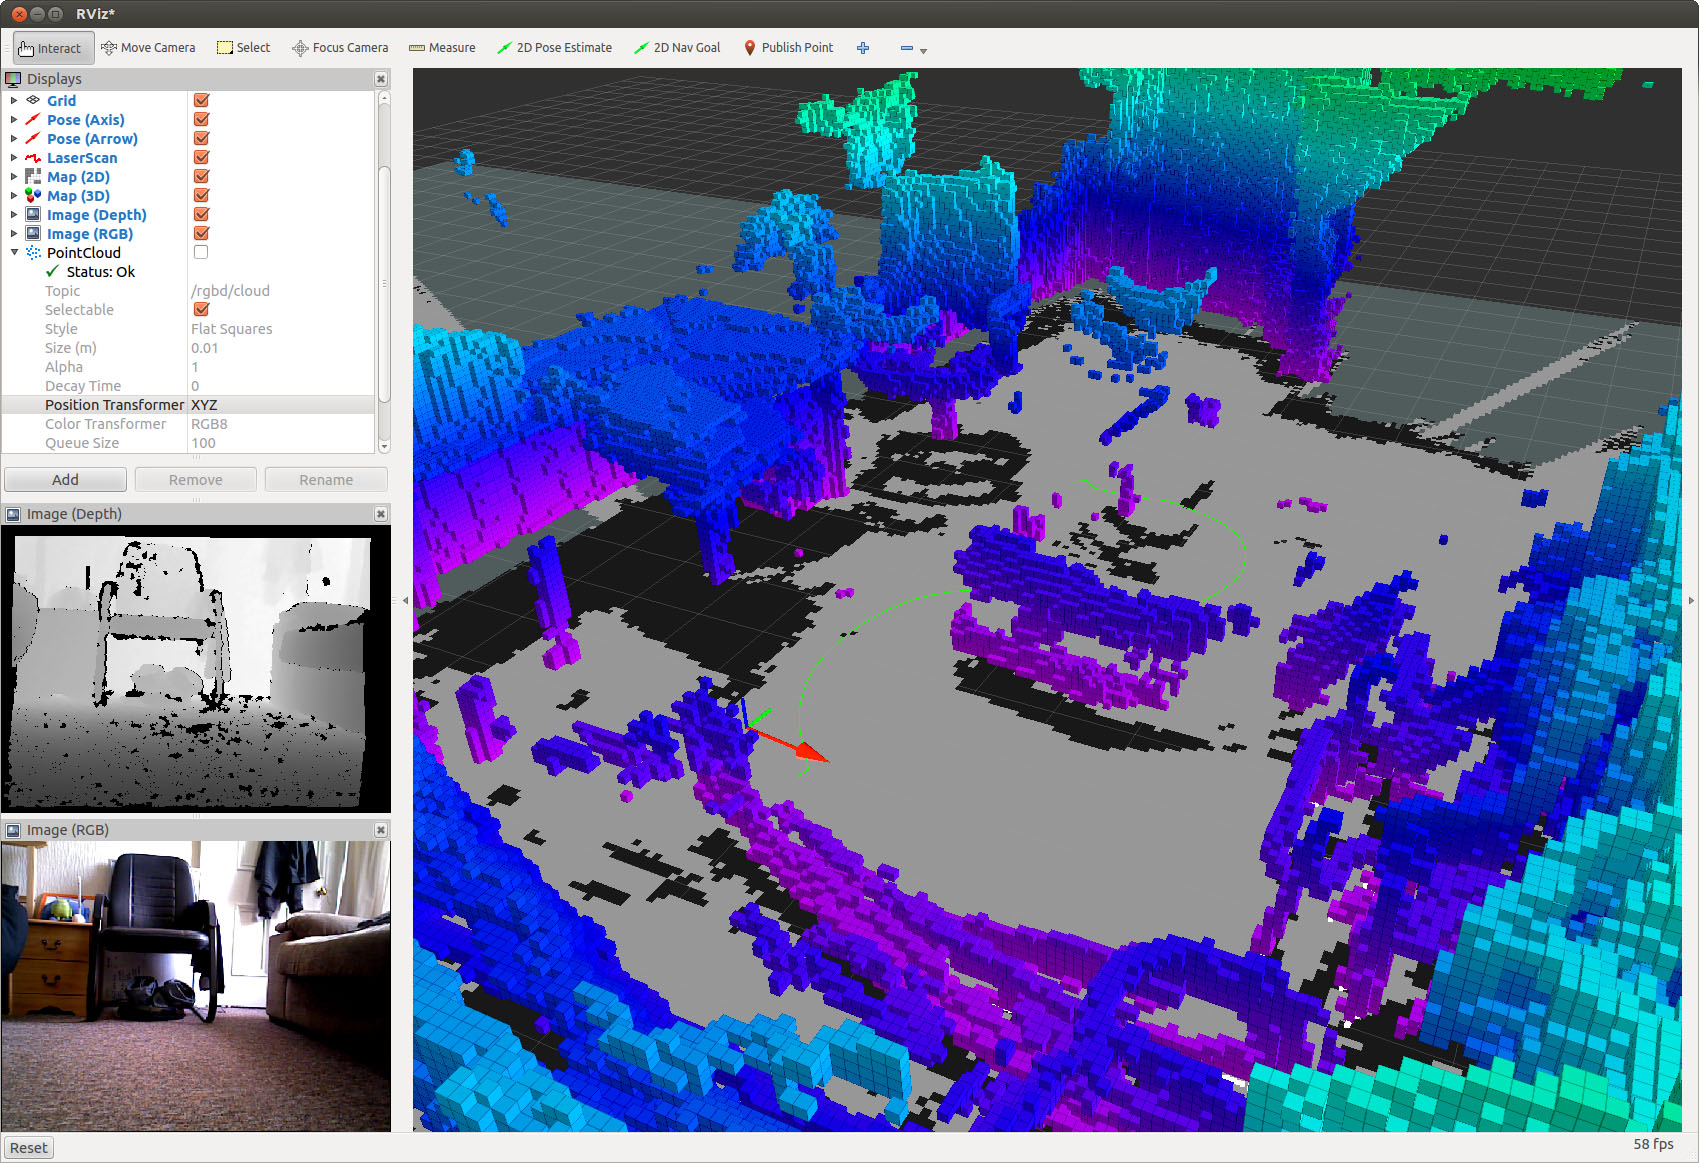
\includegraphics[width=15cm]{rviz1.jpg}
    \caption{An example configuration of RViz, specifically in the configuration used for the robot control system. The two image feeds from the camera can be seen on the left hand side, along with the configuration window for each visualisation. The main window shows the space in which the robot is operating, where a number of visualisations show the positioning and mapping facilities of the system. The green line, in particular, represents the current navigational path that the robot will follow.}
    \label{fig:rviz}
\end{figure}

\emph{rviz} is a highly configurable program for displaying visualising data from topics in a control system. It can be considered the hub of interactivity for the robot control system, allowing a user to control and understand the underlying control system. Visualisations are made possible through a plugin system, a number of which are distributed with the package. These plugins provide visualisations for a number of common messages \cite{ros_wiki_rviz_datatypes}, examples of which are shown in \autoref{fig:rviz}. A major advantage of this plugin concept is that new visualisations can be developed an integrated with \emph{rviz} easily without having to modify the core of the program itself. This may be necessary if a control system implements some new type of message, for example. In particular, many community-provided packages implement new visualisations for their custom messages.

Additionally, it is possible to interact with the control system through \emph{rviz} through \emph{interactive markers} \cite{ros_wiki_rviz_intmark}. A user is able to move or rotate these markers on-screen, depending on the configuration, which can be used to control a corresponding robot limb, for example. The same markers can also be used to set navigational waypoints which a robot can then follow. Internally, marker data is transmitted and received through the usual topic system.

\subsubsection{tf: Transforming Between Various Coordinate Frames}
A common problem in robotics is the need to transform between different coordinate frames. For example, a number of laser rangefinders may be placed in varying positions around the the base of a robot. The incoming range data from a rangefinders will be relative to its origin. Should it be necessary to find the distance from the base of the robot to a nearby wall in sight of the rangefinder, for example, some arithmetic must be performed to calculate the distance, based on the physical offsets between the base and the rangefinder. Rather than performing these calculations manually each time, ROS provides a standard solution for achieving this through the \emph{tf} package \cite{ros_wiki_tf}. An annotated example of these concepts is shown in \autoref{fig:tf}.

\begin{figure}[!h]
    \centering
    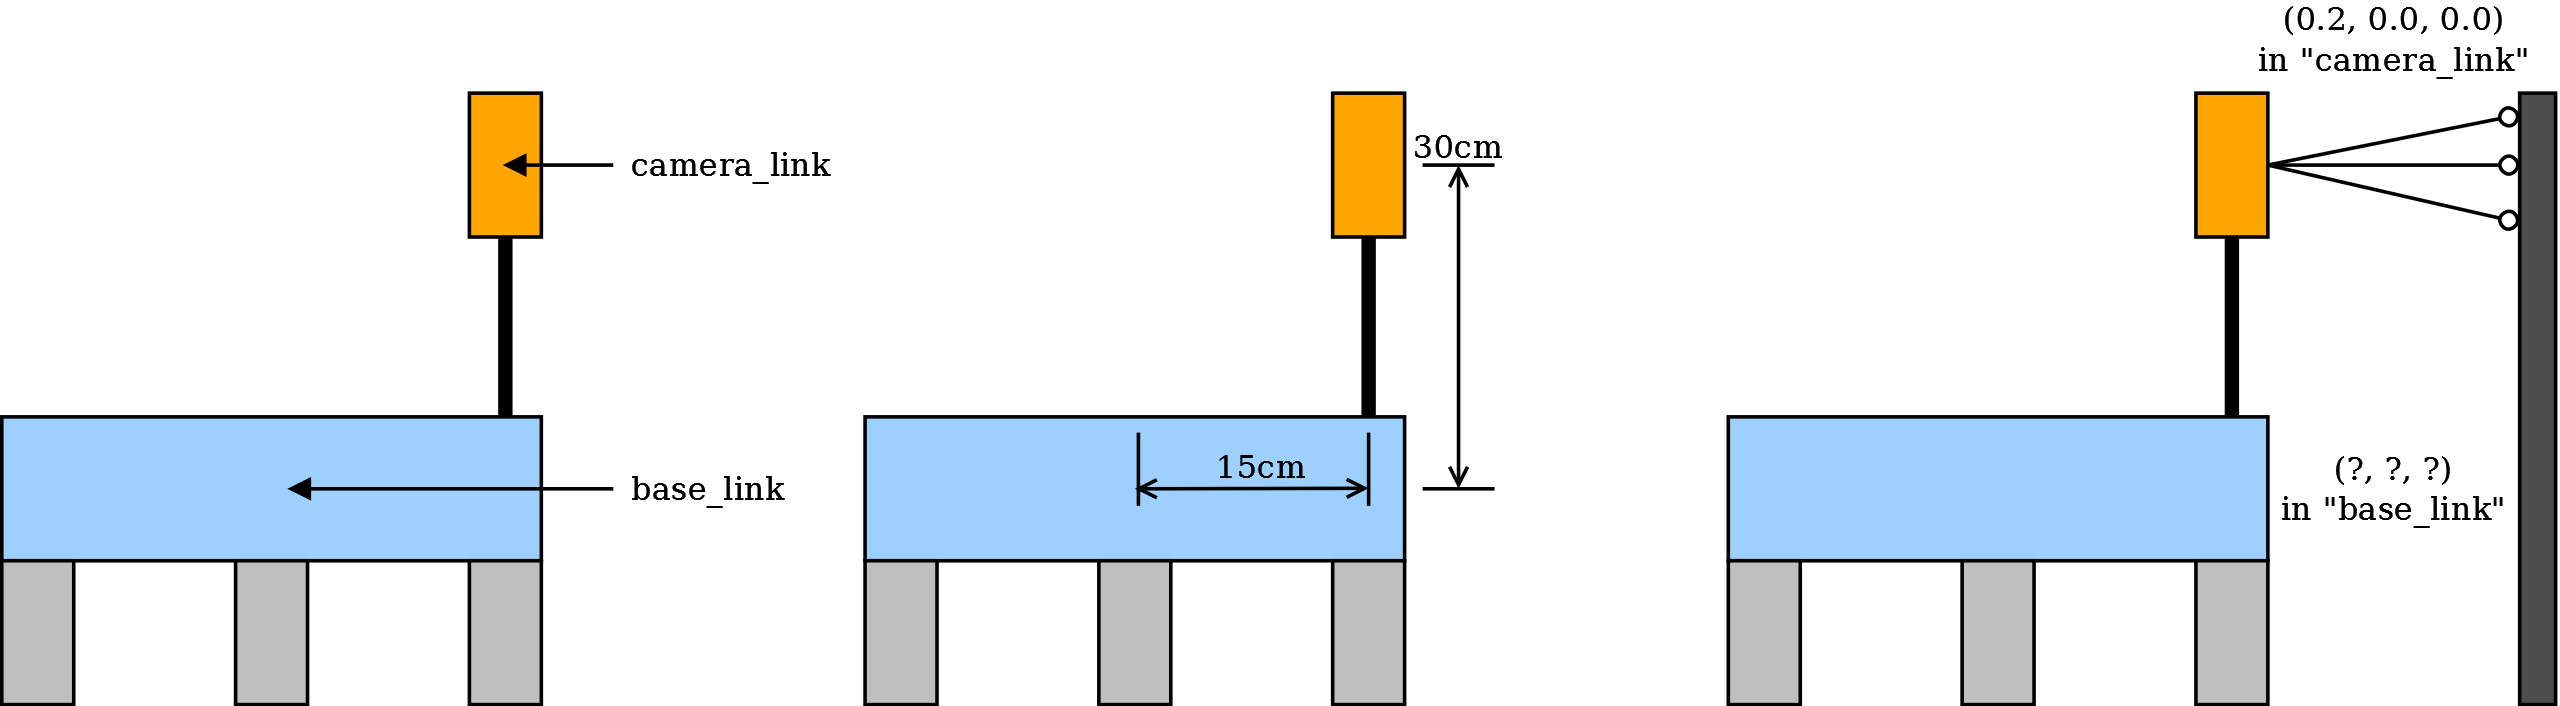
\includegraphics[width=17cm]{tf2.png}
    \caption{A diagram showing the necessity for some sort of transformation system, modelled after the robot. In the first picture, the two transformation links for this robot are shown. In the second picture, the distances between the origins of the two transformation links are shown. Specifically, it can be said that \texttt{camera\_link} is positioned at an offset of $(0.15, 0.30, 0)$ meters relative to \texttt{base\_link}. The inverse of this is also true in that \texttt{base\_link} is positioned at an offset of $(-0.15, -0.30, 0)$ meters relative to \texttt{camera\_link}. In the third picture, points detected on a wall at a distance of $(0.2, 0, 0)$ meters relative to the camera are shown. By applying the transformation offsets between \texttt{camera\_link} and \texttt{base\_link}, it is possible to calculate the distance of the points relative to base of the robot. Through simple arithmetic via the transform, it can be shown that the points are at a position of $(0.35, 0.3, 0)$ meters relative to the base of the robot.}
    \label{fig:tf}
\end{figure}

The relations between different coordinate frames and their transformations are represented in a tree-like hierarchy where each node corresponds to a particular coordinate frame. A fixed frame is used as the root of this node representing a coordinate frame from which the rest can relate to. This fixed frame can represent the environment around a robot, for example. By traversing through this tree, it is possible to calculate positions in one coordinate frame relative to another. An example transform tree is shown in \autoref{fig:tf_tree}.

\begin{figure}[!h]
    \centering
    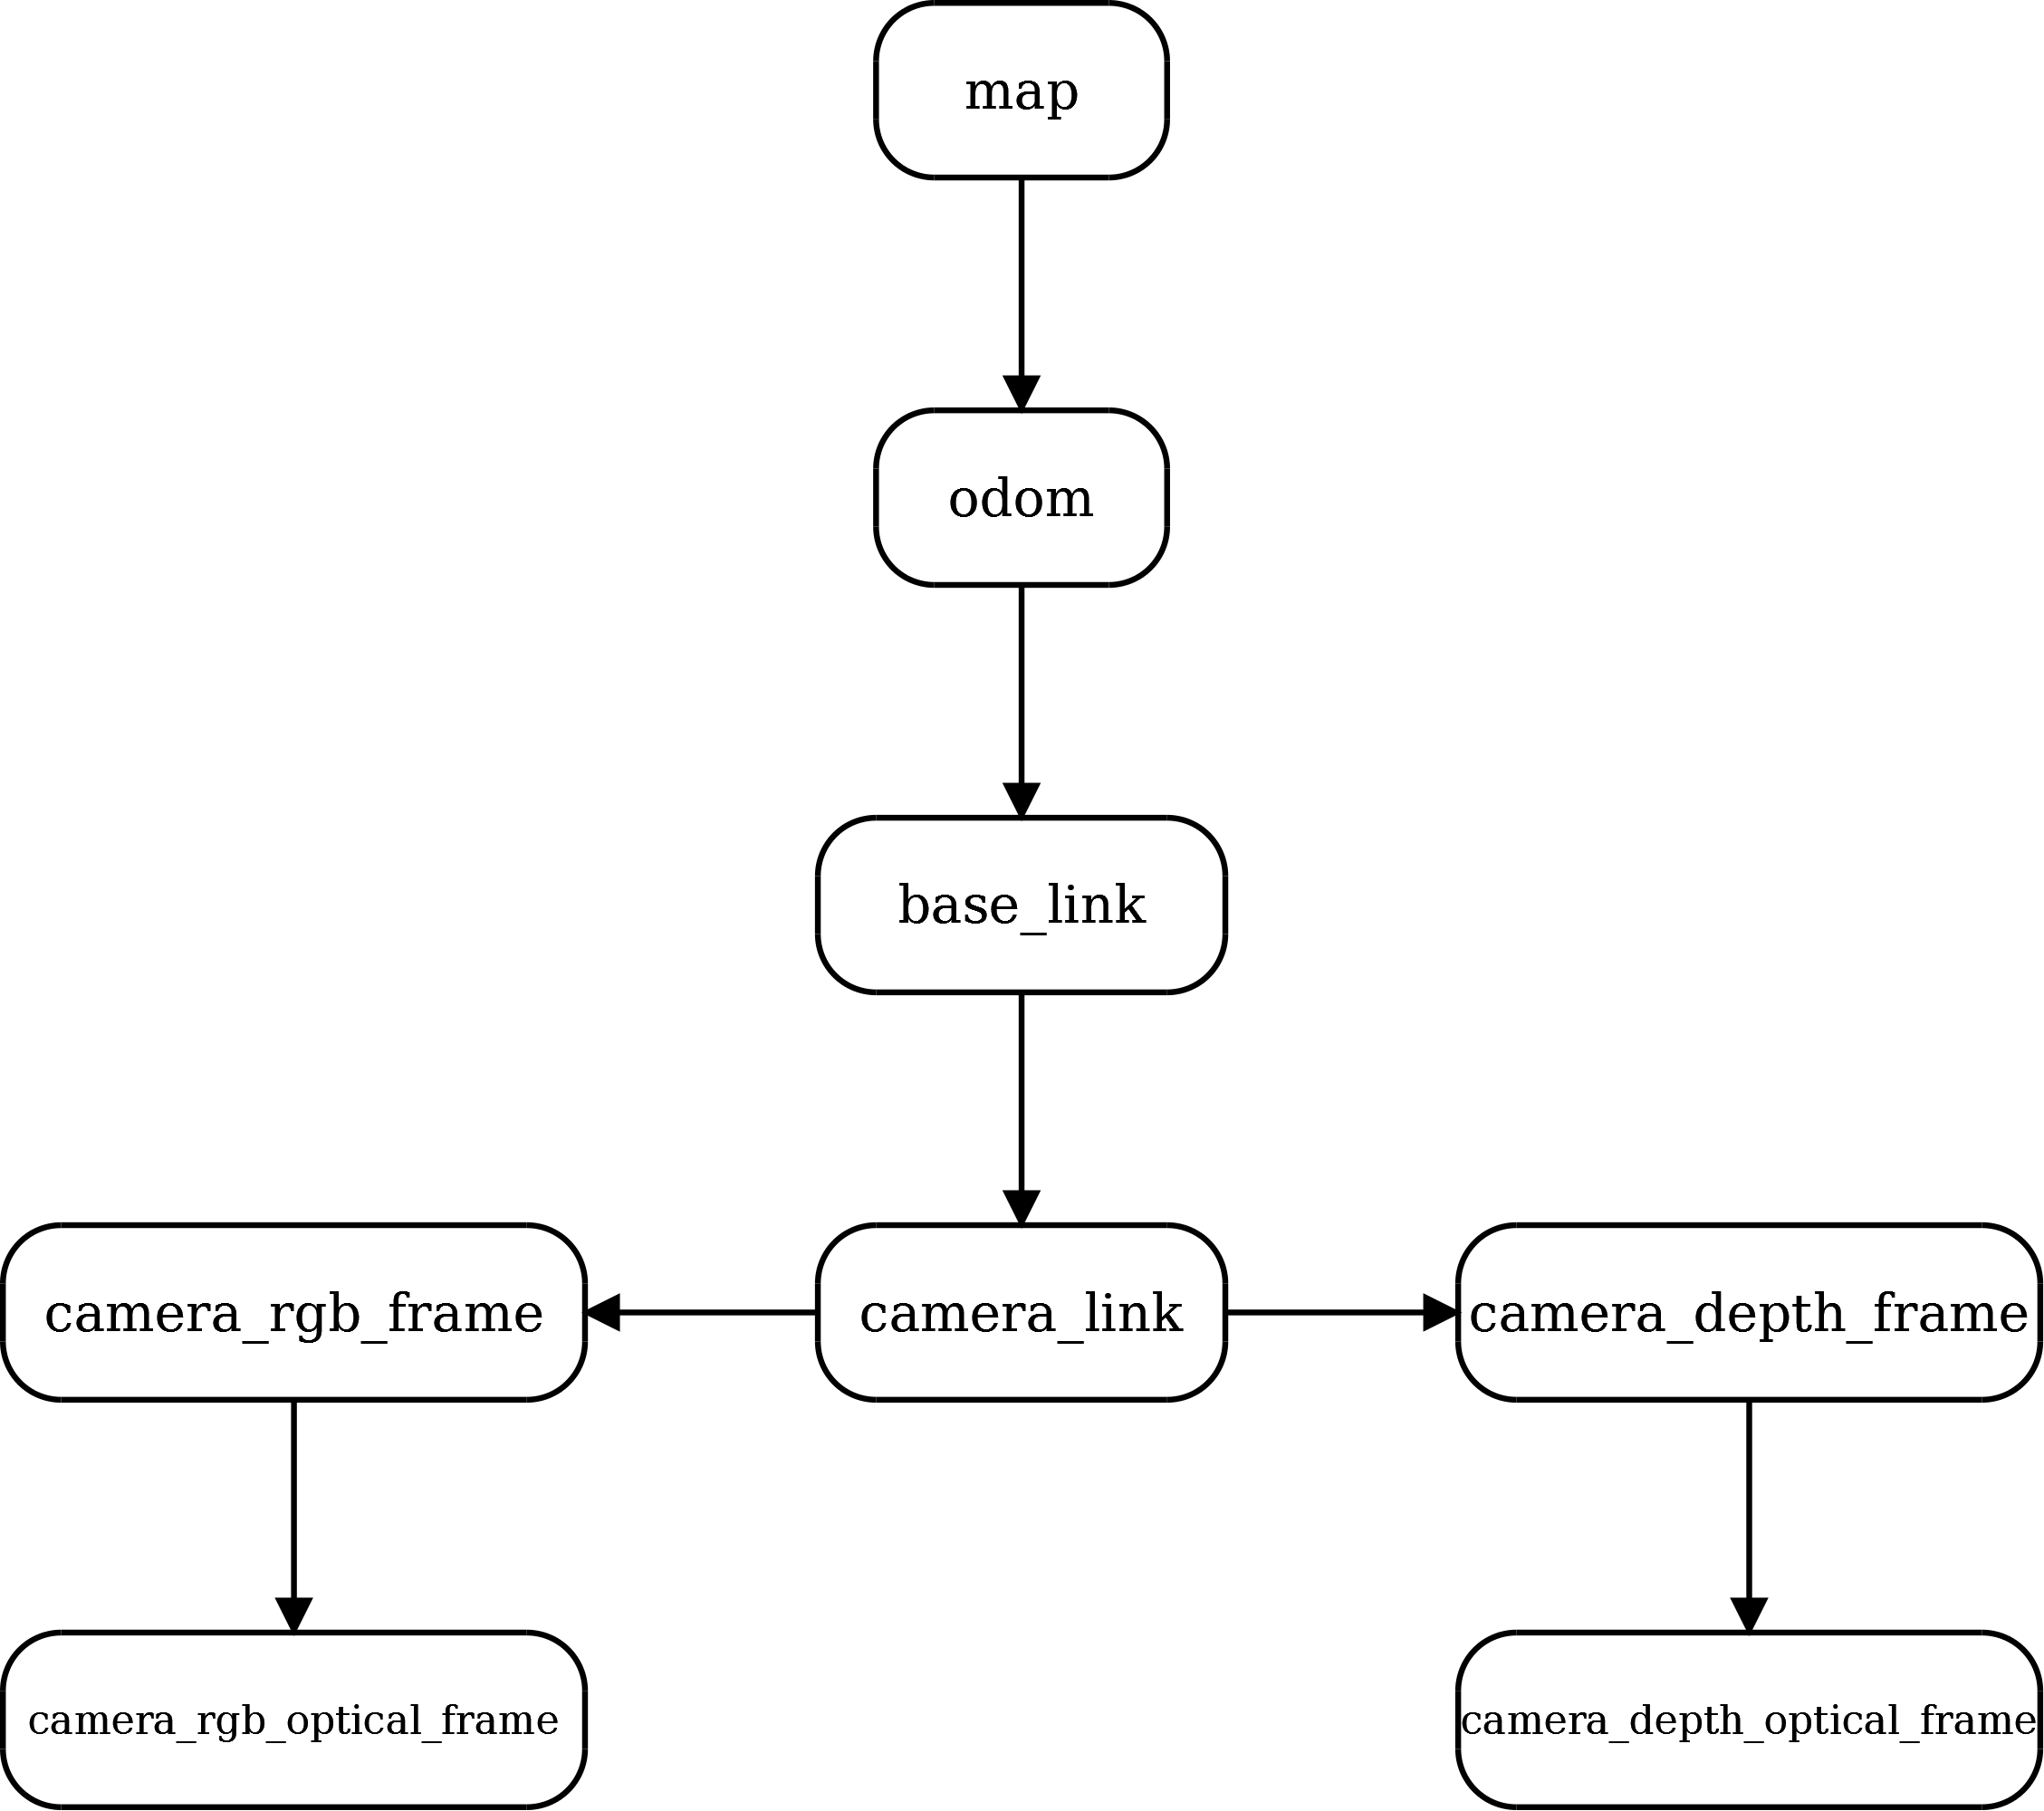
\includegraphics[width=10cm]{tf.png}
    \caption{A simplified diagram of a transform tree modelled after the implemented robot control system. Grey boxes represent a particular transform, while arrows between boxes indicate a transform relation. Each transform provides its position and rotation in space relative to the previous transform. For example, it is possible to get the position of the RGB-D camera relative to the environment by requesting a transform between \texttt{camera\_link} and \texttt{map}. The \emph{tf} system will compute the resulting position based on the supplied transforms, working backwards through the hierarchy as necessary.}
    \label{fig:tf_tree}
\end{figure}

The \emph{tf} package has a variety of useful features. Transform positions are cached throughout run-time such that it is possible to request positions at times in the past. Additionally, a number of nodes are available in the \emph{tf} package that can publish static transforms between coordinate frames. In the example shown in \autoref{fig:tf}, one would use these nodes to publish the offsets between base of the robot and the camera as they remain in the same relative position throughout run-time.

%%%%%%%%%%%%%%%%%%%%%%%%%%%%%%%%%%%%%%%%%%%%%%%%%%%%%%%%%%%%%%%%%%%%%%%%%%%%%%%%%%%%%%%%%%%%%%%%%%%%

\section{Hardware}

The robotic hardware used in this project is relatively straightforward, consisting of a number of off-the-shelf components. The robot is a hexapod-type in that it has six limbs. Each limb has three joints which can be rotated as shown in \autoref{fig:hexapod_dof}, giving three degrees-of-freedom per limb. 

\begin{figure}[!h]
    \centering
    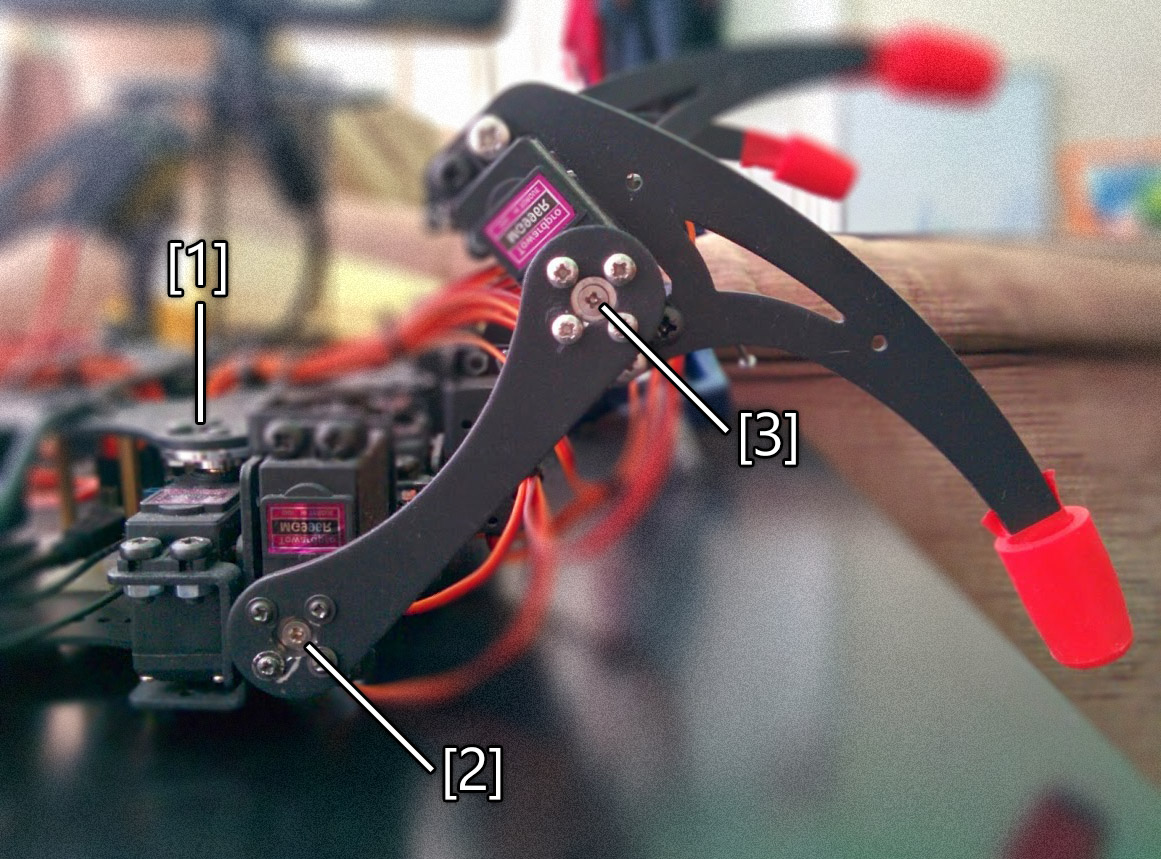
\includegraphics[width=12cm]{hexapod_joints}
    \caption{This annotated photograph shows the three degrees-of-freedom available to each limb on the robot. Joint 1 provides horizontal rotation to the leg, which can be used to push the robot forward. Joints 2 and 3 provide vertical rotation which can be used to adjust the robot's height, as well as being used for locomotion in general.}
    \label{fig:hexapod_dof}
\end{figure}

In its current state, the robot has no wireless capability and, thusly, operates in a tethered manner. A bundle of cables protruding from the rear end of the unit connects the on-board hardware to a nearby power source and computer.

\subsection{RGB-D Camera}
The primary sensor in the system is an \emph{ASUS Xtion Pro Live} RGB-D camera, which is very similar to the \emph{Microsoft Kinect}. The key functionality of this camera is that it provides a depth data feed, giving a range of values indicating the distances to the objects in front of it. The images shown in \autoref{fig:rgbd_images1} show an example of the output provided by this camera. A combination of an infra-red grid emitter and infra-red sensor is used to calculate the distances of any nearby objects, however we need not concern ourselves with the particular intricacies of its operation.

\begin{figure}[!h]
    \centering
    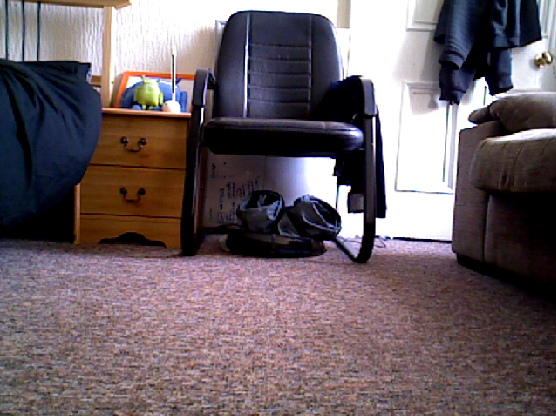
\includegraphics[width=8cm]{rgbd_rgb2.jpg}
    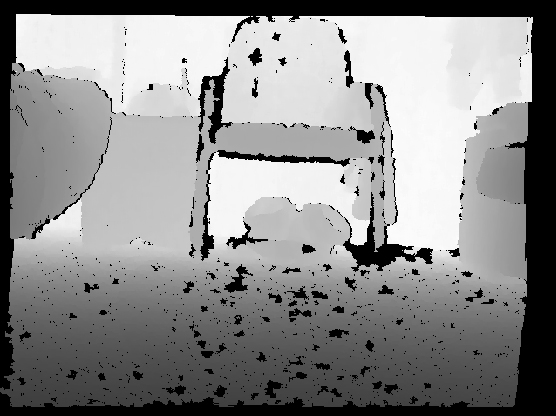
\includegraphics[width=8cm]{rgbd_depth2.jpg}
    \caption{Example imagery from the RGB-D camera mounted on top of the robot as given by the \texttt{openni2\_camera} package. The image on the left shows the RGB output from the camera. The image on the right shows the depth output interpreted as a monochrome image.}
    \label{fig:rgbd_images1}
\end{figure}

It should be noted that the depth detection range is not unlimited. The specification for the device states that the range of detection is from $0.8$m to $3.5$m \cite{xtion_spec}. Objects that are too close will cause significant errors in the resulting depth imagery, while objects that are too far away will simply not be detected. Additionally, the device has problems with reflective surfaces, again causing significant errors in the resulting depth imagery. These issues do not effect the colour feed.

The advantages this particular sensor provides over the \emph{Kinect} is mostly physical, specifically weight and footprint. The \emph{Kinect} has a motorized base which allows the device to be tilted upwards and downwards through software, in comparison to the \emph{Xtion} which has a simple hinge that must be rotated by hand. This feature is unnecessary in this use case and adds a significant amount of weight. Additionally, the \emph{Kinect} is intended to be a consumer device and, thus, has a much striking product design. However, this striking design comes at the cost of making the device much larger in general. As space on the robot's base is at a premium, this makes the \emph{Xtion} much more favourable.

Should one wish to develop for the \emph{Xtion} in general, they must use the \emph{OpenNI} framework which is a ``standard framework for 3D sensing'' \cite{openni_site}. In particular, the \emph{Xtion} requires the use of \emph{OpenNI2} which is the second iteration of this framework. The framework encapsulates much of the complex hardware interaction such that it is possible to get the output imagery with relative ease. A \texttt{openni2\_camera} package exists that provides a wrapper node for this framework, such that the imagery can be accessed through standard ROS topics.

\subsection{Servos \& Servo Controller}
Each joint piece is attached to the shaft of a servomechanism (servo) to facilitate rotation. Each servo is controlled by a \emph{pulse-width modulated} (PWM) signal supplied by the controller such that the angle of the servo can be controlled precisely. Servos operate using a feedback-loop system such that the current of an internal motor is controlled, rotating the shaft to the desired position. Rotational range and speed of servos vary depending on model, but in this case the servos allow for a total rotational range of 180\textdegree.

The servos are controlled by an off-the-shelf servo controller board, specifically the \emph{ToroBot 32-channel Servo Controller}. This board, in particular, expects text-based control commands over serial, either via direct TTL or emulated over an on-board USB to TTL converter \cite{torobot_manual}. A number of commands are supported, allowing control of the position of both single and groups of servos. Additionally, a set of movements can be programmed and issued with a single command \cite{torobot_manual}. Power is also distrusted to the servos via this board.

No package that implements a driver for this particular servo controller exists within the ROS repositories, so our control system would have to implement its own.

\subsubsection{Protocol}

Commands are issued using an ASCII-based protocol via serial communication. While the servo controller supports a number of commands, only the command which rotates an individual servo is necessary. This allows for more flexibility in terms of when the rotation begins, as all servos mentioned in a group command will begin rotation at the same time.

\begin{figure}[!h]
    \centering
    \texttt{\#\(n\)\#P\(a\)T\(t\)}
\end{figure}

A rotation command is issued by sending a string in the format shown above, specifying the particular servo number ($1 \leq n \leq 32$), the target position ($1500 \leq a \leq 2500$), and the time over which the rotation should occur ($100 \leq t \leq 9999$) in milliseconds. The command is ended by a carriage return followed by a new line character. A working example is shown below, where we rotate the servo at index 1 to 90\textdegree{} over 250ms.

\begin{figure}[!h]
    \centering
    \texttt{\#1\#P2000T250}
\end{figure}

It should be noted that the parameter for the target position is actually the pulse-width duration (in milliseconds) that is sent to the servo rather than an actual angle. Duration ranges can very per manufacturer however there is a common standard such that 1.5\textmu s corresponds to 0\textdegree{} and 2.5\textmu s correspond to 180\textdegree. These are the minimum and maximum possible values for this controller. 

%%%%%%%%%%%%%%%%%%%%%%%%%%%%%%%%%%%%%%%%%%%%%%%%%%%%%%%%%%%%%%%%%%%%%%%%%%%%%%%%%%%%%%%%%%%%%%%%%%%%

\section{Existing Robot Control Systems}

A number of ROS-based control systems exist for prefab robots. Some examples of these include the \emph{PR2} by \emph{Willow Garge} for which ROS was originally created \cite{ros_pr2}, the \emph{Jaguar} by \emph{Dr Robot Inc} \cite{jag}, and the \emph{TurtleBot} \cite{turtlebot}. These robots are purchasable from the manufacturer in an already assembled form, where the manufacturer has also implemented a control system. This allows any buyer to get started implementing interesting behaviours on top of this system without having to worry about movement, navigation, etc. These systems target their corresponding hardware platforms specifically and, as such, cannot be adapted for use with our hexapod-type robot. Regardless, these systems can be used to gain an understanding of what shape a control system should take in general. Furthermore, these control systems rely on generic packages underneath which we can, indeed, leverage.

As far as could be found, there are no existing robot control systems for hexapod-type robots that are based upon ROS. By doing a web search, it is possible to find numerous forum posts by hobbyist roboticists suggesting that some are being developed, but none in an official research sense. Additionally, these posts are usually dead end leads in that no source code, or even further information in general, can be found. Furthermore, no existing robot control systems for any hexapod-type robots exist within the ROS repositories. It is for this reason, that we must design and develop our own control system.

%%%%%%%%%%%%%%%%%%%%%%%%%%%%%%%%%%%%%%%%%%%%%%%%%%%%%%%%%%%%%%%%%%%%%%%%%%%%%%%%%%%%%%%%%%%%%%%%%%%%

\section{Visual Interpretation}

A number of research papers were found relating to the use of RGB-D cameras for localisation and environment mapping, however these papers dealt with the specifics of the algorithms used rather than their usage in general \cite{correa2012mobile, biswas2012depth, cunha2011using}. Furthermore, none of these projects targeted ROS in particular and thus would require us to implement them by hand. These algorithms are particularly complex and, as such, were outside the scope of this project. The use of any existing package that implemented this sort of functionality would be favoured instead.

Two packages were found that deliver this functionality. Specifically, \texttt{ccny\_rgbd} and \texttt{octomap\_mapping} \cite{ccny_rgbd, ros_wiki_octomap}. These provided a means for position estimation and environment mapping respectively through simplified interfaces. The particulars of these packages will be detailed in the implementation section.

%%%%%%%%%%%%%%%%%%%%%%%%%%%%%%%%%%%%%%%%%%%%%%%%%%%%%%%%%%%%%%%%%%%%%%%%%%%%%%%%%%%%%%%%%%%%%%%%%%%%

\section{Summary}

To summarise this background information, ROS provides us with the following useful features which we can leverage while implementing our robot control system.

\begin{itemize}
    \item A means of dividing complex functionalities into separate tasks through the use of nodes.
    \item A means of asynchronous communication between these nodes through topics using standard data structures.
    \item A method to group these nodes into subsystems through packages.
    \item A standard way of programatically launching large groups of nodes while being able to group them into namespaces. Additionally, a means of providing parameters to these nodes such that they can be reconfigured as necessary.
    \item A method of transforming between various positional frames on the robot.
    \item A user interface that can be used to visualise sensor data and provide control inputs to the control system.
\end{itemize}

Combined, these features greatly simplify the development process by offloading much of the difficult work onto the framework itself. Furthermore, a number of standard and community-provided ROS packages already provide us with the following functionality:

\begin{itemize}
    \item Drivers for the RGB-D camera which publishes the imagery on a number of topics.
    \item A visual odometry system that can be used to estimate the robot's position in the environment using camera imagery.
    \item A mapping system capable of interpreting the environment using camera imagery, such that obstacles can easily be detected.
    \item A full navigational suite capable of path planning and robot control.
\end{itemize}

While these packages get us a significant way to completing the system, we must still implement the following functionality ourselves:

\begin{itemize}
    \item Drivers for controlling the on-board servo controller.
    \item A method of locomoting the robot---e.g, through some walk gait.
\end{itemize}

Additionally, a number of existing robot control systems exist within the ROS repositories but these target specific robots and, thus, cannot be adapted for use with our hexapod. A number of visual interpretation methods were researched but the specifics of these were too complex for the scope of this project. Instead, we rely on a number of community-provided packages to give us this functionality.
\chapter{Approach}
\label{chap:approach}

To evaluate the usefulness of ROS, we set out to build a ROS-based robot control system, targeting the hexapod as its primary hardware platform. A number of increasingly complex requirements were necessary for this system to function correctly.

Throughout, an attitude of code re-use was taken, relying on any existing nodes and packages where possible. It was assumed that these requirements would be otherwise unachievable in this project's time frame without the help of this vast package repository. As there are many ROS packages available that perform similar tasks, it was necessary to choose and compare these packages where appropriate. 

%%%%%%%%%%%%%%%%%%%%%%%%%%%%%%%%%%%%%%%%%%%%%%%%%%%%%%%%%%%%%%%%%%%%%%%%%%%%%%%%%%%%%%%%%%%%%%%%%%%%

\section{Requirements}

The requirements for the control system can be divided into four key categories as explained in the following sections.

\subsection{Hardware Operation}

To achieve any real-world interaction, the system had to be capable of interfacing with our target hardware platform. Drivers in some form were required to allow communication to both the servo controller and the RGB-D sensor. Ideally, these should transmit and receive on topics using common data types.

\subsection{Locomotion}

As this robot relies on walking motions for movement, which consists of a complex sequence of servo rotations, some abstraction of this process was required. Specifically, it was necessary to be able to control both the linear and rotational velocities of the robot without knowledge of the underlying servo movements. For this, walking gaits would have to be investigated such that an appropriate one could be chosen.

Some calibration process was also necessary. Due to the manner in which the servos connect to their respective joint sections, it is extremely difficult to align them such that they are perfectly straight. A method was required such that offsets can be applied to any positions sent to the servo controller, on a per-servo basis. To make this process easier, some tool to adjust these offsets was required.

Additionally, a method of manually controlling the robot was needed. This would allow for simple testing before any autonomous behaviour was added, as well as acting as a general safety net should anything go wrong.

\subsection{Sensing}

By using information received from the attached RGB-D sensor, the system had to be be able to interpret the world around it. Specifically, we looked to build up a map of the immediate surrounding area such that it was possible to detect any objects and obstructions.

A method of inferring the position of the robot relative to the rest of the world was also required. Wheeled robots have an advantage in that they are able to apply rotary encoder techniques, allowing them to extrapolate their current position relative to a starting position. As this is a walker-style robot, this presented a particularly difficult challenge.

\subsection{Navigation}

Finally, the robot had to be capable of some autonomous behaviour. For this, autonomous navigation was chosen as it would be a stepping stone to any further behaviours. By using the interpreted visual data, the robot had to be able to navigate its environment to reach some particular target, avoiding any obstructions and obstacles where necessary. To achieve this, we would require a complete working integration of the aforementioned goals.

%%%%%%%%%%%%%%%%%%%%%%%%%%%%%%%%%%%%%%%%%%%%%%%%%%%%%%%%%%%%%%%%%%%%%%%%%%%%%%%%%%%%%%%%%%%%%%%%%%%%

\section{Design}
\chapter{Implementation}

%%%%%%%%%%%%%%%%%%%%%%%%%%%%%%%%%%%%%%%%%%%%%%%%%%%%%%%%%%%%%%%%%%%%%%%%%%%%%%%%%%%%%%%%%%%%%%%%%%%%

This chapter will document the implementation process of the robot's systems.

At the time of writing, the most recent version of ROS is \emph{Hydro}. A machine running \emph{Ubuntu 12.04 LTS}, the primary distribution for Hydro, was used for all development.

%%%%%%%%%%%%%%%%%%%%%%%%%%%%%%%%%%%%%%%%%%%%%%%%%%%%%%%%%%%%%%%%%%%%%%%%%%%%%%%%%%%%%%%%%%%%%%%%%%%%

\section{Architecture}

Through the use of packages, we split the robot system into a number of systems, grouped by one larger system. Specifically, 

%%%%%%%%%%%%%%%%%%%%%%%%%%%%%%%%%%%%%%%%%%%%%%%%%%%%%%%%%%%%%%%%%%%%%%%%%%%%%%%%%%%%%%%%%%%%%%%%%%%%

\section{Hardware Operation}

% FIXME: Maybe put this elsewhere?
From the outset, it was known that the depth sensor relied on the \emph{OpenNI2} library and already had a supporting package. However, no such packages existed for the servo controller.

\subsection{RGB-D Camera Driver}

A wrapper for the \emph{OpenNI2} library is provided by the \texttt{openni2\_camera} \cite{ros_wiki_openni2_camera} and \texttt{openni2\_launch} \cite{ros_wiki_openni2_launch} packages. The former provides a single nodelet which acquires and publishes the image data, whereas the latter provides a means for starting that nodelet.

This driver publishes image data from the camera on a number of different topics, with varying data types. Only two of these are particularly useful to us, however. The topic \texttt{/camera/rgb/image} provides the general optical feed from the camera, and the topic \texttt{/camera/depth/image} provides the depth feed from the camera, both of message type \texttt{Image}. Some example output from these topics is shown below. 

While the depth feed can be interpreted as an 8-bit monochrome image for displaying on-screen, the image is actually given in a 16-bit format, where each pixel value represents the distance from the sensor in millimeters. Additionally, the depth data is available in a point cloud format, published on \texttt{/camera/depth/points} as \texttt{PointCloud2} messages.

Understanding these package was rather troublesome, as both the wiki and GitHub pages documenting them were (and still are) completely blank. Instead, the documentation for a similar set of these packages for the first version of \emph{OpenNI}, named \texttt{openni\_launch}, was used \cite{ros_wiki_openni_launch}. Regardless, there was little difficulty in setting this package up.

\subsection{Servo Driver}

While there were already drivers for the RGB-D sensor, the case was not the same for the servo controller. For this, a custom node had to be developed.

%%%%%%%%%%%%%%%%%%%%%%%%%%%%%%%%%%%%%%%%%%%%%%%%%%%%%%%%%%%%%%%%%%%%%%%%%%%%%%%%%%%%%%%%%%%%%%%%%%%%

\section{Locomotion}

Strictly, only joints 1 and 2 are necessary for a tripod gait. Joint 3 can be locked, perhaps as a single solid piece of material, such that a right angle is formed between the foot and leg sections. This provides a stable stance for the robot to balance upon as it pushes itself forward between each cycle.

\subsection{Limb Controller}
\subsection{Limb Calibration Tool}
\subsubsection{Usage}

\subsection{Tripod Gait Walker}
\subsection{Joystick Controller}

%%%%%%%%%%%%%%%%%%%%%%%%%%%%%%%%%%%%%%%%%%%%%%%%%%%%%%%%%%%%%%%%%%%%%%%%%%%%%%%%%%%%%%%%%%%%%%%%%%%%

\section{Sensing}

openni2 originally, ccny\_rgbd \cite{ccny_rgbd} provides some clean up features.

\subsection{Visual Odometry}

ccny\_rgbd \cite{ccny_rgbd} was used.

\subsection{Environment Mapping}

ocotomap

\subsubsection{Alternatives}

SLAM, but expects laser scan.

%%%%%%%%%%%%%%%%%%%%%%%%%%%%%%%%%%%%%%%%%%%%%%%%%%%%%%%%%%%%%%%%%%%%%%%%%%%%%%%%%%%%%%%%%%%%%%%%%%%%

\section{Navigation}

Built in stack.

\subsection{Path Planning}

\chapter{Evaluation}
\label{chap:evaluation}

%%%%%%%%%%%%%%%%%%%%%%%%%%%%%%%%%%%%%%%%%%%%%%%%%%%%%%%%%%%%%%%%%%%%%%%%%%%%%%%%%%%%%%%%%%%%%%%%%%%%

A number of experiments were conducted to evaluate the correctness of the implemented robot control system. The robot control system was ran in its entirety on a high-end machine running Ubuntu Linux 12.04 LTS. Specifically, the machine has an \emph{Intel Core i7 3770K} clocked at \emph{4.5Ghz} paired with \emph{16GB} of memory. An attempt to run the control system on an \emph{Apple MacBook Pro} was made, which has an \emph{Intel Core i5 3239M} clocked at \emph{2.6Ghz} paired with \emph{8GB} of memory, but the machine could not achieve the performance necessary for good operation.

\begin{figure}[!h]
	\centering
	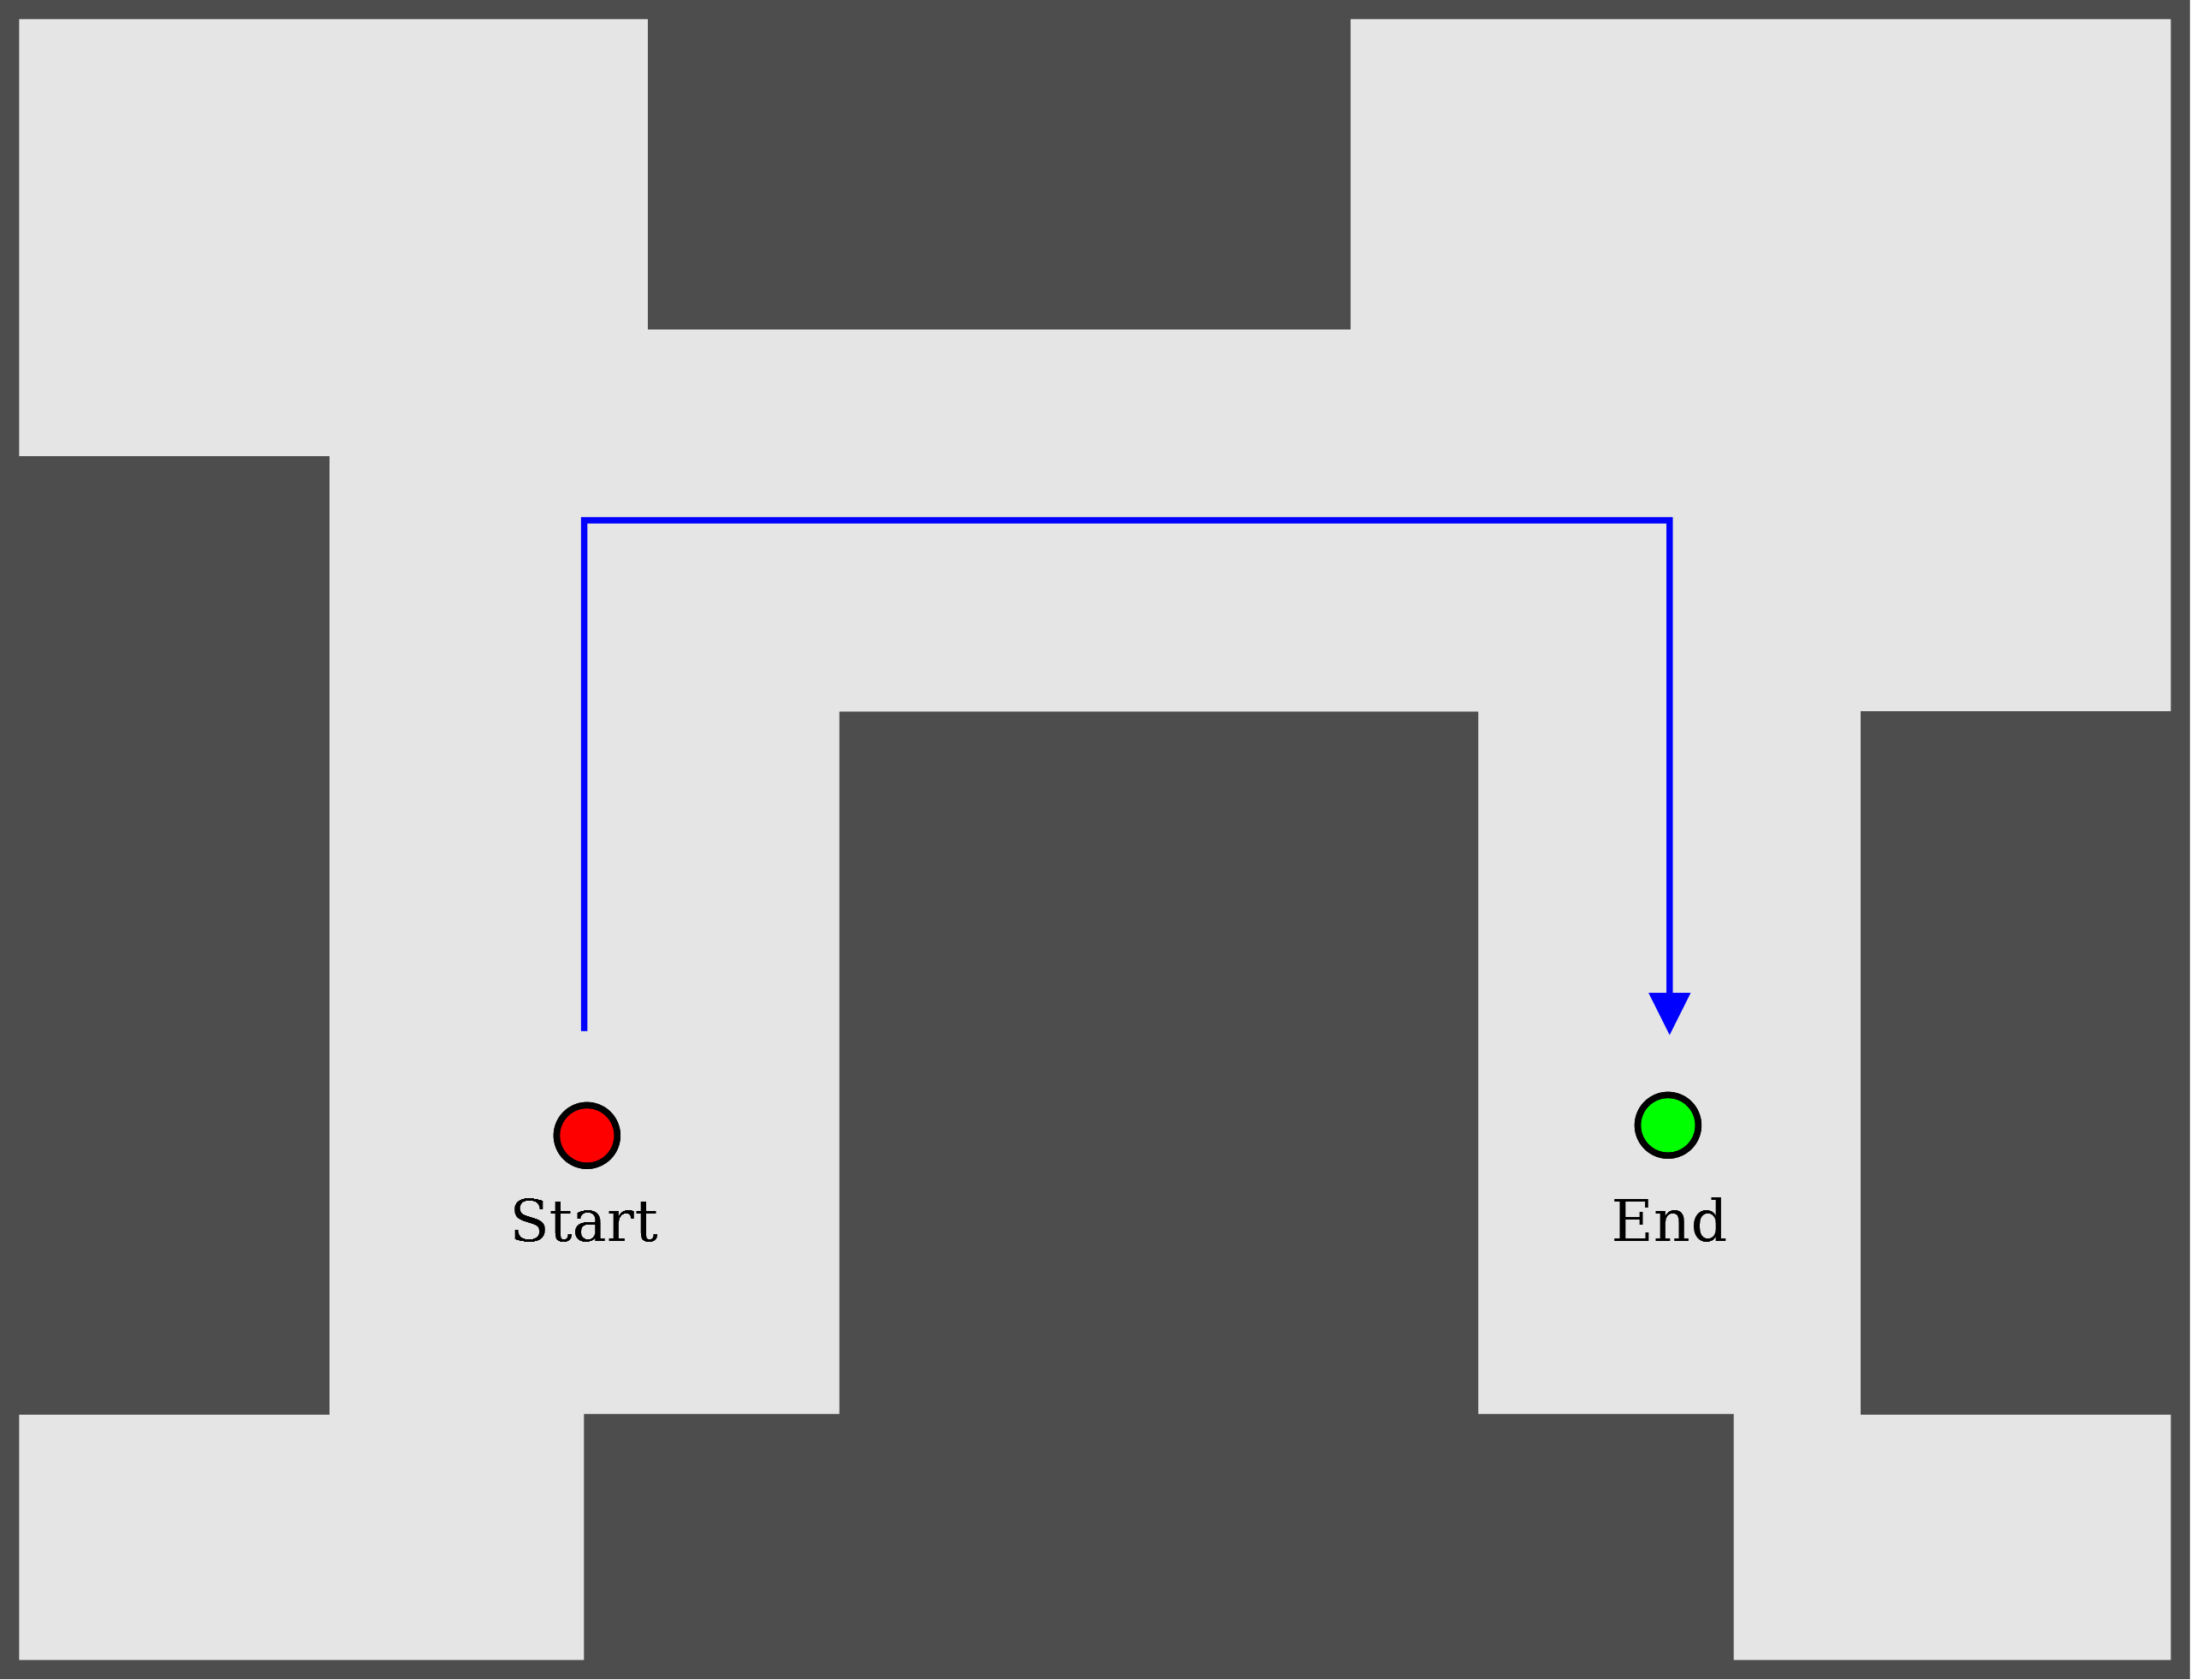
\includegraphics[width=12cm]{plan.png}
	\caption{A diagram of the general layout of the test environment---not to any particular scale. Darkened shapes indicate large obstacles that the robot must detect and avoid. The robot was placed at the starting point at the beginning of each test. The end point indicates the target goal for the navigational tests along with an ideal path.}
	\label{fig:eval_plan}
\end{figure}

Testing took place in a large environment as shown in \autoref{fig:eval_plan}. This environment contained a number of everyday obstacles with varying shapes, colours and textures. All tests were ran under ideal lighting conditions---i.e., full natural light---where possible. This ensured that the RGB-D camera provided the highest of quality images which would have a knock-on effect for the visual odometry and mapping subsystems.

\section{Hardware Interaction}

These experiments were created to test the correct function of the hardware interaction systems, specifically the RGB-D camera driver and the servo driver.

\subsection{RGB-D Camera Driver}

The RGB-D camera driver, provided by the \texttt{openni2\_driver} and \texttt{openni2\_launch} packages, was tested by observing output through \emph{rviz}. A \emph{rviz} configuration was made that would show both the colour and depth video feeds from the camera, taken from the \texttt{/camera/rgb/image} and \texttt{/camera/depth/image} topics. As this is a standard package, it was expected that it would function as intended without any issues.

That said, a peculiar fault was discovered in that the device would show itself to be disconnecting and reconnecting repeatedly while running. Throughout this, many USB timeout messages and similiar errors were shown in the Linux \emph{message buffer}---shown by \texttt{dmesg}. The cause of the issue turned out to be that, simply, the USB cable from the computer to the camera was too long. The USB specification states that devices running in USB 2.0 mode---which is the case for the \emph{Xtion}---may have a maximum cable length of $5$m \cite{usb_spec}. The cable had been extended to allow a larger movement distance but the resulting cable length was now $6.5$m long, as the \emph{Xtion} already had a $1.5$m cable attached.

Following this discovery, the cable was trimmed to $5$m and, as a result, the driver functioned correctly as intended.

\subsection{Servo Driver}

To test the servo driver for the system, which is implemented as a custom \texttt{servo\_controller} node, we ran the following experiments. Each experiment was implemented as a custom node would would then be ran alongside the driver nodes to execute the test. Correctness of results were determined by visual observation---i.e., looking to see if joints moved as intended. 

\subsubsection{Rotation of a Single Servo}

This first experiment was designed to confirm correct behaviour when moving only one servo at a time. To elaborate further, we aimed to check the following:

\begin{description}[labelindent=\parindent]
	\item[Hardware Communication] \hfill \\
	If the servo controller was receiving any of the serial output sent by the \texttt{servo\_controller} node whatsoever, the on-board indication LED would flash with each message. This would have shown that the servo controller is receiving serial output as intended. No flashing LED would have indicated some general issue with the serial communication components.

	\item[Topic Reception] \hfill \\
	If the \texttt{servo\_controller} node was receiving \texttt{ServoCommand} messages sent on its \texttt{direct} topic, we expected some sort of change in system state in general---even if that involved the node crashing. No change would have indicated a problem with the topic subscriber within the node.

	\item[Index, Angle \& Duration Conversion] \hfill \\
	Should the formulae for converting from the units specified in the \texttt{ServoCommand} message to those specified by the servo controller's protocol be correct, we would have expected the specified servo to move the correct angle over the correct duration. Any deviation from this would have indicated some mathematical error in the formulae.
\end{description}

To implement this particular experiment, a \texttt{servo\_controller\_test\_single} node was created. This node requests four movements from each servo sequentially in a continuous loop at various angles and durations, pausing for one second between each. A listing of these movements is shown in \autoref{tab:servo_controller_eval}.

\begin{table}[!h]
	\centering
	\begin{tabular}{ c c c }
		\toprule
		\textbf{Movement} & \textbf{Angle} & \textbf{Duration} \\
		\midrule

		$1$ &
		$90$\textdegree{} &
		$1.00$s \\

		$2$ &
		$180$\textdegree{} &
		$0.25$s \\

		$3$ &
		$0$\textdegree{} &
		$0.50$s \\

		$4$ &
		$90$\textdegree{} &
		$0.75$s \\
		\bottomrule
	\end{tabular}
	\caption{A listing of movements made for each servo in the single servo rotation test. These movements are applied to each servo in a continuous loop with a one second delay between each movement.}
	\label{tab:servo_controller_eval}
\end{table}

The \texttt{servo\_controller} node and \texttt{servo\_controller\_test\_single} node were launched and the robot observed. Prior to this, the robot was placed upon a pedestal to ensure that the limbs could rotate freely without unintentionally moving the robot. As expected, each servo rotated as intended to the correct angles and durations, thus showing the implementation was functional as required.

\subsubsection{Simultaneous Rotation of Multiple Servos}

The second experiment was designed to confirm correct behaviour in the case of multiple servos being moved simultaneously---i.e., where movement is requested for a number of servos such that the movement durations overlap. This was an essential requirement as no walk gaits would be possible without.

To implement this experiment, the \texttt{servo\_controller\_test\_single} node from the previous experiment was adapted to create a new \texttt{servo\_controller\_test\_multiple} node. This node performed the same set of movements but on all servos simultaneously rather than sequentially.

The \texttt{servo\_controller} node and \texttt{servo\_controller\_test\_double} node were launched and the robot observed, while the robot was placed on a pedestal as before. It was from this test that the necessity for a small delay between each serial communication was discovered. Without this delay, servos would either not rotate whatsoever or abort their requested rotation part-way through. During this, the indication LED on the servo controlled would also light up solidly, rather than flash as it does during normal operation. It was presumed that this meant there was some sort of communication error, perhaps as commands were being sent too quickly for the on-board microcontroller to process them. After adding an delay of $0.1$s, the problem immediately subsided. This was further reduced to a minimum delay of $0.003$s by trial-and-error, preventing any knock-on effects for commanding nodes. As mentioned in the implementation section for the \texttt{servo\_controller} node, no source code is available for the microcontroller software so no further diagnosis can be made. 

Following this modification, the test ran as intended, thus showing the implementation was functional as required.

\section{Locomotion}

These experiments were created to evaluate that the systems designed to handle locomotion operated correctly. Specifically, we aimed to test the correct function of the limb controller, the limb calibration tool, and the walk controller.

\subsection{Limb Controller}

The limb controller, implemented as a custom \texttt{limb\_controller} node, was tested in a manner similar to the servo controller. The servo controller test nodes were adapted to send messages to the limb control topics, rather than the topic used to control the servos directly. Through running the same set of tests, the limb controller was shown to function correctly.

\subsection{Limb Calibration Tool}

The implementation of the limb calibration tool is fairly trivial and was used throughout the evaluation of the control system and as such, no particularly rigorous testing was performed. Testing was performed throughout the implementation process and the node was found to work as intended. Generally, the joint servos had to be re-calibrated during each session of operation, as the particular servos used are rather inaccurate. A number of realisations came about during its use.

In particular, it was found that achieving an accurate calibration through manual manipulation was essentially impossible. There are no markings on the robot with which the current angles of joints can be compared, so calibration was usually done by eye alone. Using a measuring implement, such as a protractor, was also infeasible as the physical geometry of the robot prevents such devices from aligning correctly with the servo axles. This issue could be alleviated by adding additional sensors on the robot---e.g., gyroscopes and accelerometers---such that calibration could be performed automatically or to, at the very least, give some notion of the stability of the robot.

Additionally, it was found that the servos would not rotate by small increments but only when it had reached a certain threshold away from its current position---e.g., if a servo is currently at $90$\textdegree{} then it will not rotate immediately until a rotation of $\pm2$\textdegree{} is requested whereupon it will ``snap'' into position. The particular threshold seemed to vary wildly depending on the particular servo \emph{and} its position. This ramifications of this were such that while a limb may seem calibrated, it could in fact be out of alignment by this threshold. This would only become apparent when larger rotations were made.

In general, both of these issues could be solved be utilising more accurate (and accordingly more expensive) servos---software can only correct for hardware problems up to a point.

\subsection{Tripod Gait Controller \& Gamepad Controller}

To test the tripod gait controller, implemented by the \texttt{walk\_controller} node, we conducted the following set of experiments. These would confirm that the implemented tripod gait cycle was correct and resulted in motions as intended. Specifically, we would test that the gait worked correctly for forward motions, angular motions and a combination of both motions. Manual control would be used throughout the test, given by the \texttt{gamepad\_controller}, providing confirmation that it too was functioning correctly. Tests would involve observing the robot visually as it moved around.

\subsubsection{Linear Motion}

The first test involved simply moving the robot back and forth in a straight line from its starting position. The left analogue stick on the controller was pushed upwards and downwards, signifying a forward and backwards movement. This was done for a few minutes to ensure there were no problems. As expected, the robot moved as intended without issue.

\subsubsection{Angular Motion}

The second test involved rotating the robot in place. The right analogue stick on the controller was pushed left and right, signifying anti-clockwise and clockwise rotations. Again, this was done for a number of minutes to ensure that there were no problems. As expected, the robot rotated as intended.

\subsubsection{Combined Linear and Angular Motion}

The third test involved supplying commands for both linear and angular motions simultaneously, such that the robot would move in a curved path. This was essentially a combination of the previous two tests. Both the left and right analogue sticks on the controller were moved in varying combinations of positions. The expected outcome was that the robot should push forward or backward while also turning to one side.

It was through this test that the necessity to apply some sort of equal ratio formula to the swing angles was found. Originally, both linear and angular movement angles were simply added together based on the requested velocities---i.e., $v_x \times \texttt{swing\_angle} + v_\theta \times \texttt{swing\_angle}$. This meant that both full linear and angular movements were requested, the resulting angles sent to the servos would be twice the specified maximum---i.e., $2 \times \texttt{swing\_angle}$. This was a rather nasty problem as it caused the legs of the robot to collide and get stuck inside one another.

The solution was to utilise ratios such that the maximum angle sent to the servos could only be \texttt{swing\_angle}, as described in great detail in the implementation section. After applying this correction, the robot could move around correctly as intended. However, while this correction prevents the legs from colliding with one another, the speed at which the robot moves is somewhat reduced. If both maximum linear and angular movements are requested, the robot will only move at half the maximum speed, as the ratio formula divides \texttt{swing\_angle} equally.

\section{Sensing}

These following experiments were created to evaluate that the sensing subsystems could interpret the world around the robot via the supplied camera input. Specifically, we test both the visual odometry and mapping components of the subsystem.

\subsection{Visual Odometry}

To test the visual odometry component, which was provided by the \texttt{visual\_odometry} node in the \texttt{ccny\_rgbd} package, we ran the following experiments. These experiments involved moving the robot in various ways while observing how accurately the visual odometery component matched these movements. Experiments would be ran with both manual movement of the robot---i.e., lifting it up along a path by hand---as well as with the implemented tripod gait. The \texttt{tf\_echo} tool from the \emph{tf} suite was used to get an exact readout of the interpreted position. Each experiment was ran ten times and the resulting positions averaged.

\subsubsection{Linear Motion}

The first experiment involved moving the robot forward by one meter while observing the position given by the visual odometery component. At the start of each test, the robot was placed at the starting position shown in \autoref{fig:eval_plan} and the control system reset. The robot would then be moved forward---either manually by hand or via the tripod gait---such that the robot had moved a meter relative to this starting position. Two points were placed both at the start and end positions such that the front two feet could be aligned with them. An ideal result would have been a resulting position of $(1$m, $0$m, $0$\textdegree{}$)$.

By manual movement, the visual odometery component gave an average position of $(0.924$m, $0.004$m, $0.471$\textdegree{}$)$. Notably, the system seemed to underestimate the $x$ component by an average of $0.076$m in this case, while the $y$ component and heading remained fairly accurate. A full listing of the results can be seen in \autoref{tab:eval_vo}.

By movement via the tripod gait, the visual odometery component gave an average position of $(0.952$m, $0.013$m, $0.191$\textdegree{}$)$. Similarly, the component seemed to underestimate the $x$ component by an average of $0.048$m while the heading remains reasonably accurate. The higher $y$ component drift in this case could be due to the roughness of the walk gait. Specifically, the camera does not glide forward exactly in a straight line as it does when being moved manually through the air. Each step causes the robot shake in general as it settles into position. Again, a full listing of the results can be seen in \autoref{tab:eval_vo}.

\subsubsection{Angular Motion}

The second experiment involved rotating the robot by $90$\textdegree{} in place. As before, the robot was placed at the starting position shown in \autoref{fig:eval_plan} and the control component reset at the start of each test. The robot would then be rotated clockwise by 90\textdegree{} on the spot either either manually by hand or via the tripod gait. An ideal result would have been a resulting position of $(0$m, $0$m, $90$\textdegree{}$)$.

By manual movement, the visual odometery component gave an average position of $(0.1$m, $0.004$m, $89.296$\textdegree{}$)$. By movement via the tripod gait, the visual odometery system gave an average position of $(0.172$m, $-0.018$m, $89.284$\textdegree{}$)$. A full listing of the results from both tests can be seen in \autoref{tab:eval_vo_rot}.

In both cases, there was a significant drift in the $x$ component---a drift of $0.1$m and $0.172$m for the manual and tripod gait movements respectively---while the $y$ and $\theta_z$ components remained fairly accurate. While observing the visual odometry output through \emph{RViz}, it seemed as though the robot was rotating around a pivot rather than in place as it should be. This was a particularly troubling outcome as it had the potential to disrupt both the mapping and navigation systems, but no further diagnosis could be done without delving into the complexities of the node's source code. It is possible that a more in-depth calibration of the camera lenses is necessary, as any warping of points caused by the lens may not be taken into account. A further evaluation into this particular aspect is definitely necessary.

\subsubsection{General Commentary}

As an additional issue, should the visual odometry component be unable to find sufficient features in the images it is currently receiving---e.g., some object is obstructing the camera--- then the output position will be essentially, undefined. While an actual position is output by the component in this case, it could essentially be considered completely random and therefore useless. Additionally, when the component is able to find sufficient features once more, the position does not reset to where it was previously. At this point, the whole control component must be restarted to resume normal operations.

In general, it is was not unexpected that the visual odometry component had some positional drift. The concept of odometry is such that it provides an estimate of the current position in space, rather than an exact position. Additional sensors---e.g., laser scanners, accelerometers, GPS, etc---would be very useful in this case. A multitude of filters can then be used to combine the information such that the robot can be localized in space much more accurately.

\subsection{Mapping}

To evaluate the mapping component, we ran the following set of experiments. These experiments would confirm that the mapping component could interpret the environment surrounding the robot correctly. Additionally, they would confirm that the map can update in real-time as the robot moved around the environment. A \emph{rviz} configuration was made to display both 2D and 3D maps generated by the \texttt{octomap\_server} node, allowing us to observe the results visually.

\subsubsection{Stationary Mapping}

The first experiment involved placing the robot on the starting position as shown in \autoref{fig:eval_plan}. The robot control system would then be started, and the map output shown in \emph{rviz} observed, checking the map for general accuracy versus the real environment. No movements---apart from putting the robot into a steady standing position---would be performed.

\begin{figure}[h]
	\centering
	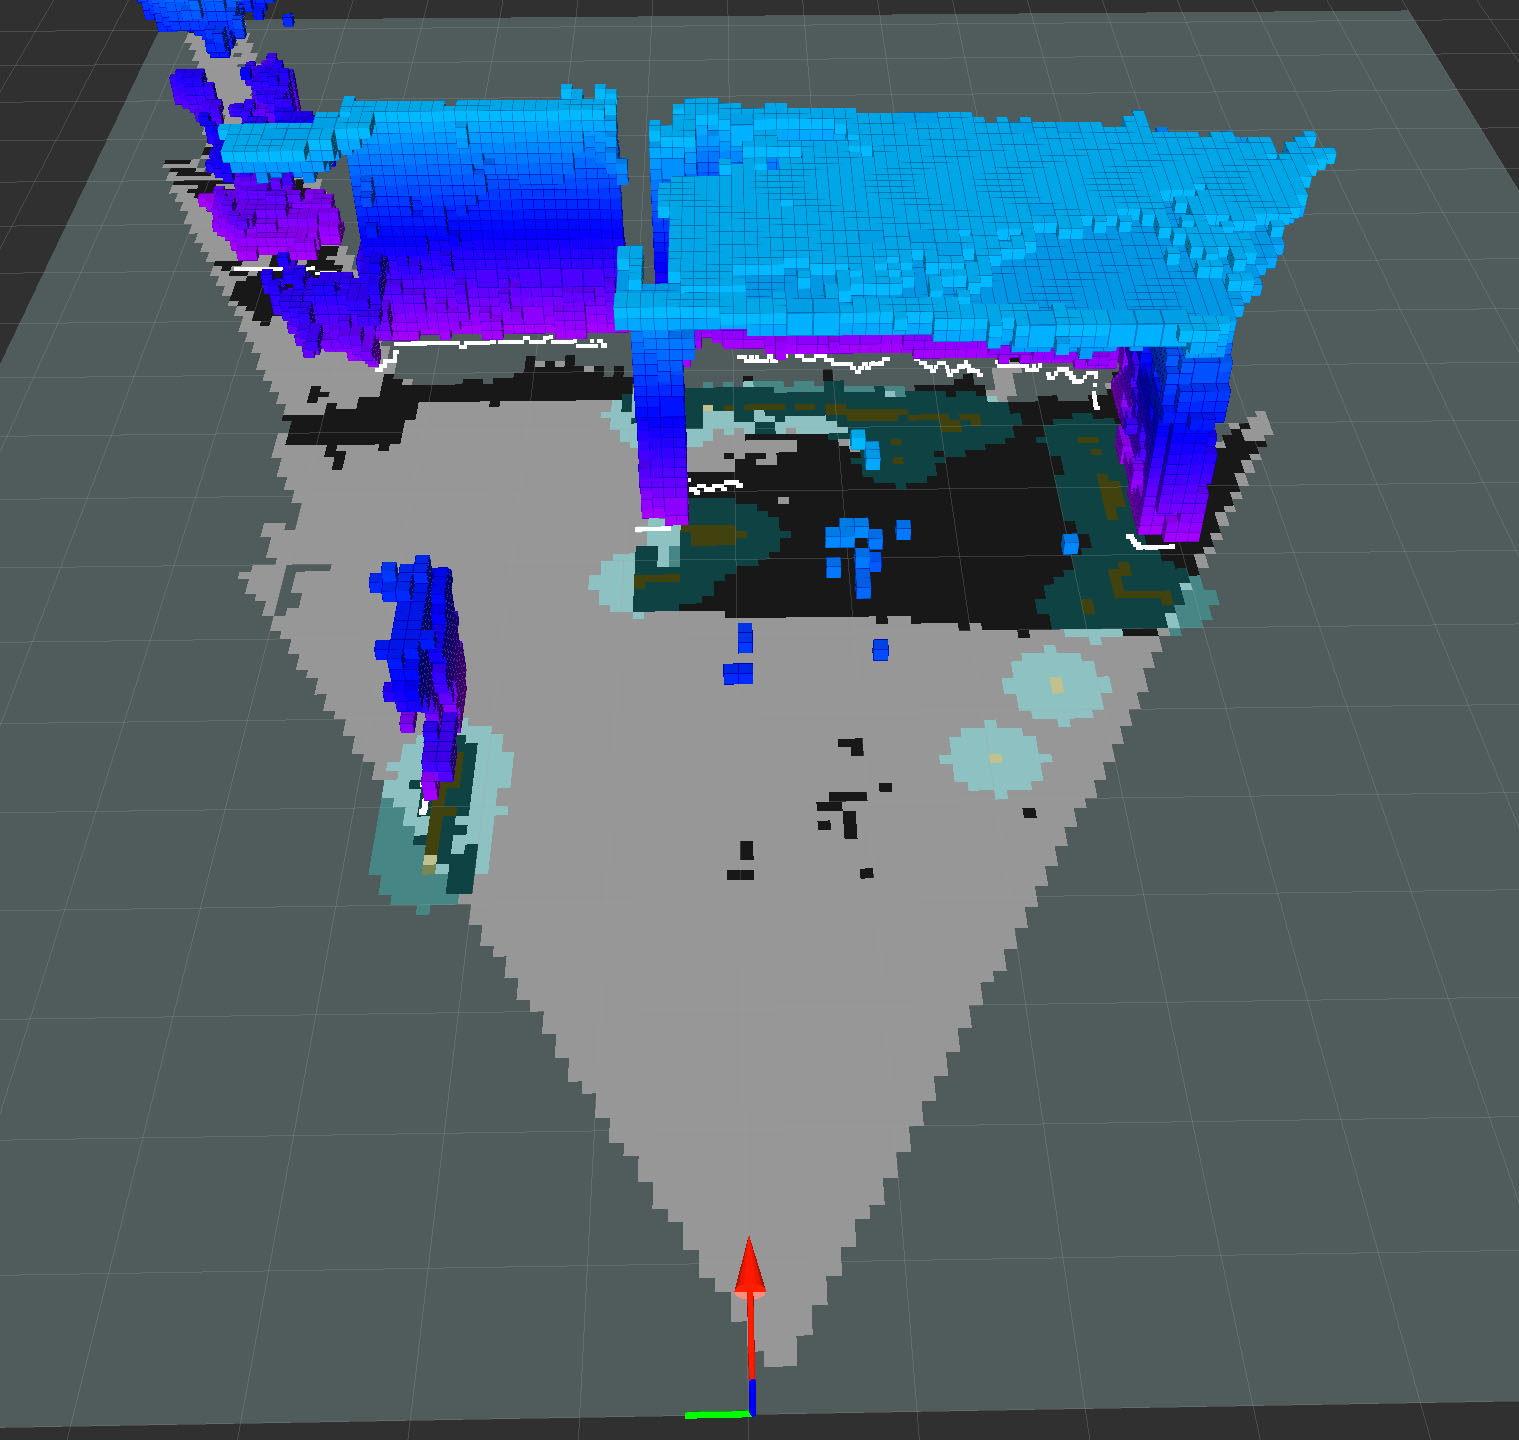
\includegraphics[width=14cm]{eval_map1.jpg} \\
	\vspace{2pt}
	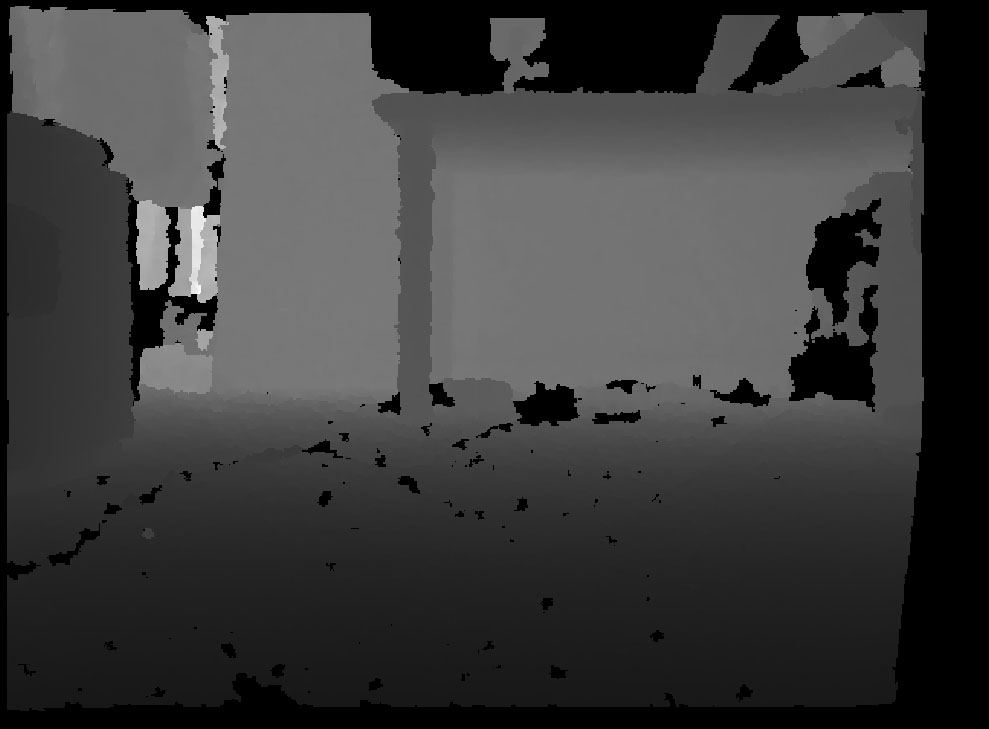
\includegraphics[width=8cm]{eval_rgbd3.jpg}
	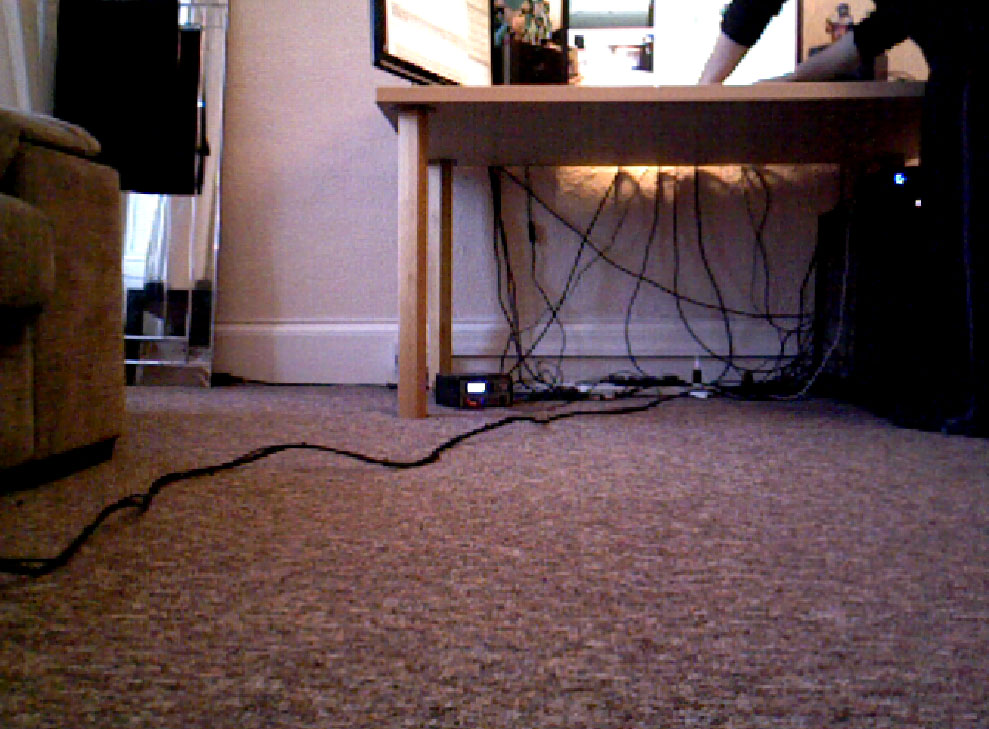
\includegraphics[width=8cm]{eval_rgbd4.jpg}
	\caption{A display of the generated map a few seconds after the robot control system has started along with the direct colour (bottom left) and depth (bottom right) outputs from the RGB-D camera. The shape of the desk and wall directly in front of the robot, as seen in the colour image, can clearly be seen in the resulting map.}
	\label{fig:eval_map_nobag}
\end{figure}

The resulting output along with raw imagery from the camera for this test as shown in \autoref{fig:eval_map_nobag}. While the map was generally accurate, there was some noise visible in the map output. It is possible that the mapping component could have erroneously detected some parts of the floor as obstacles. Regardless, they are so insignificant that the navigational systems would not have any issue with them. Thusly, this results of this experiment were deemed adequate.

\subsubsection{Stationary Mapping with an Obstacle}

The second experiment was performed in a manner similar to the previous experiment. At the start of the test, the robot was placed at the starting position and the control system started. The map output from the same \emph{rviz} configuration would then be observed. This time, however, after a few seconds an obstacle---in this case a backpack of similar height to the robot---would be placed $1$m in front of the robot. It was expected that the bag should then show up as an obstacle on the map. No movement would be performed, as before.

\begin{figure}[h]
	\centering
	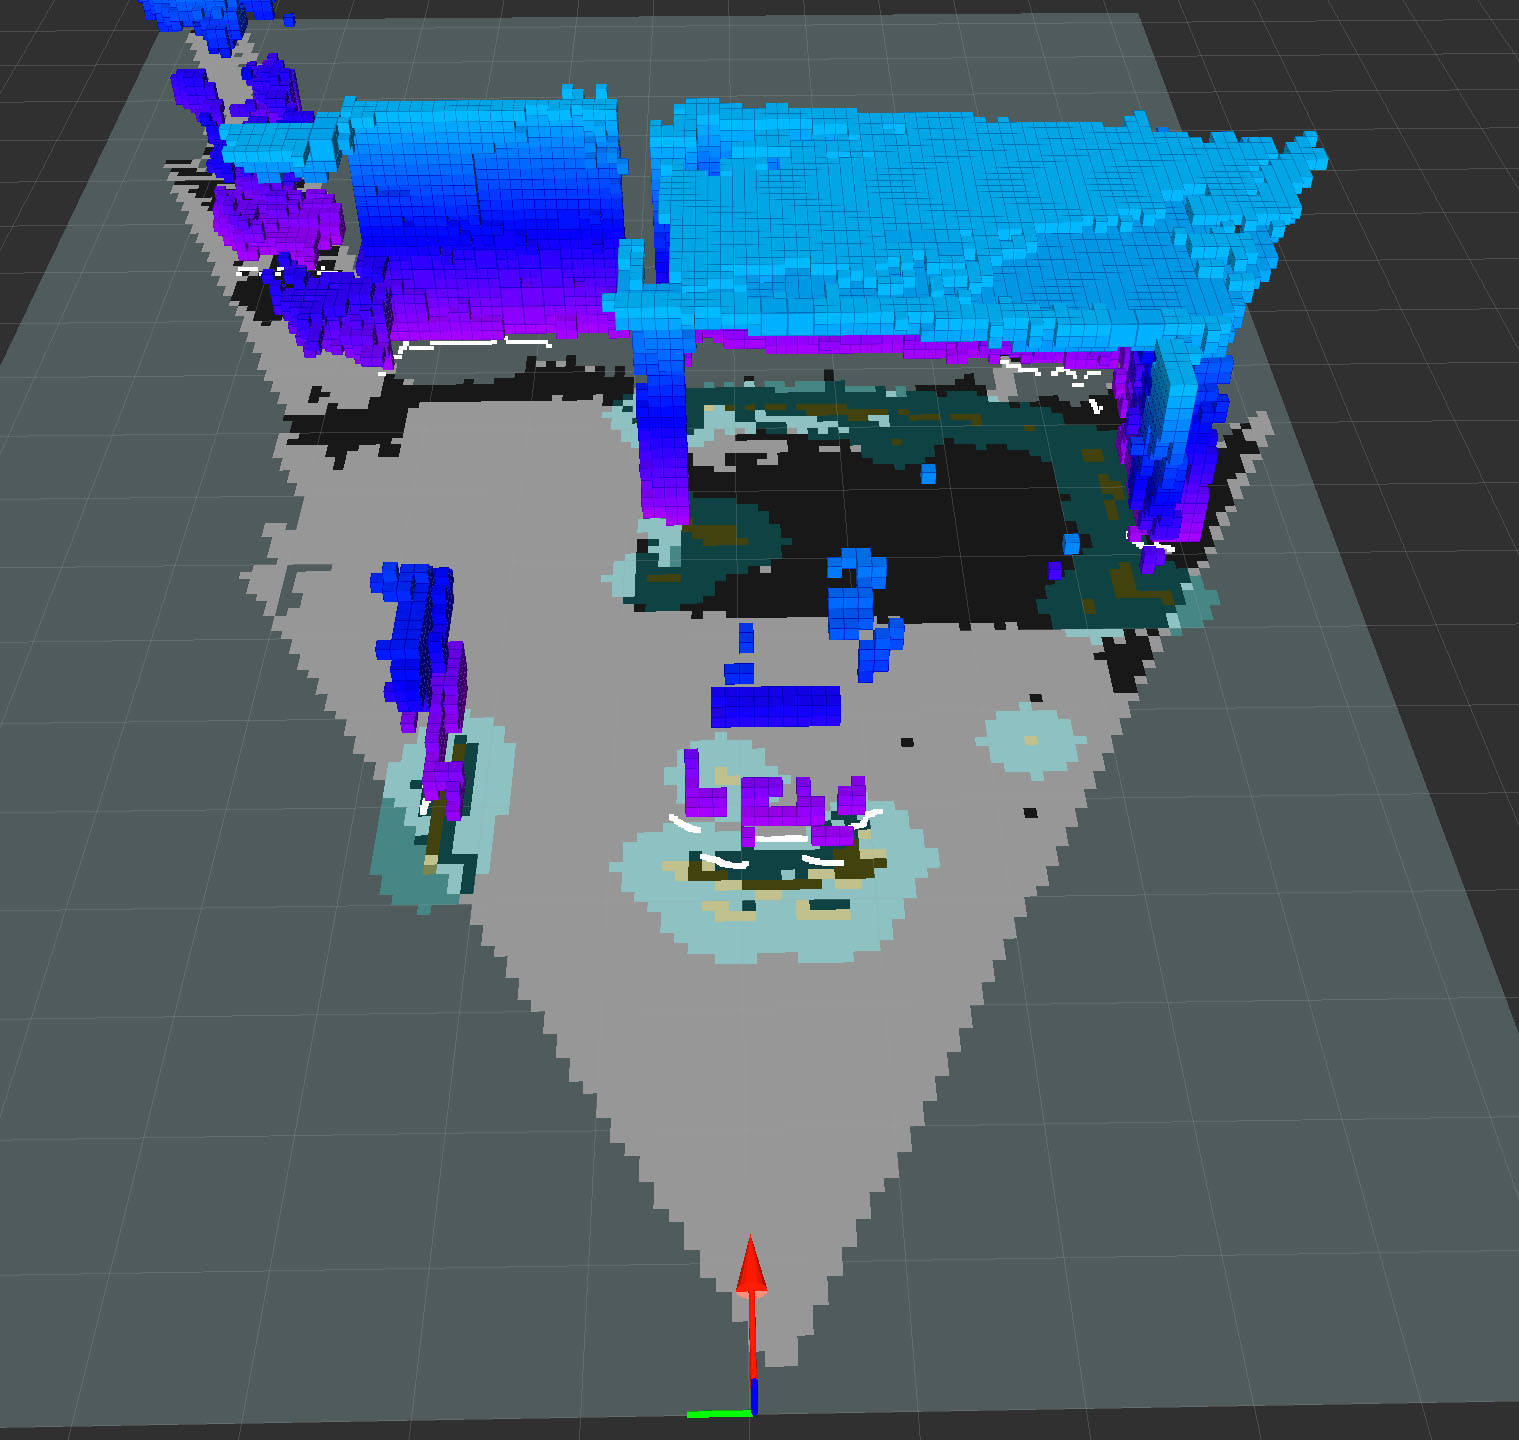
\includegraphics[width=14cm]{eval_map2.jpg} \\
	\vspace{2pt}
	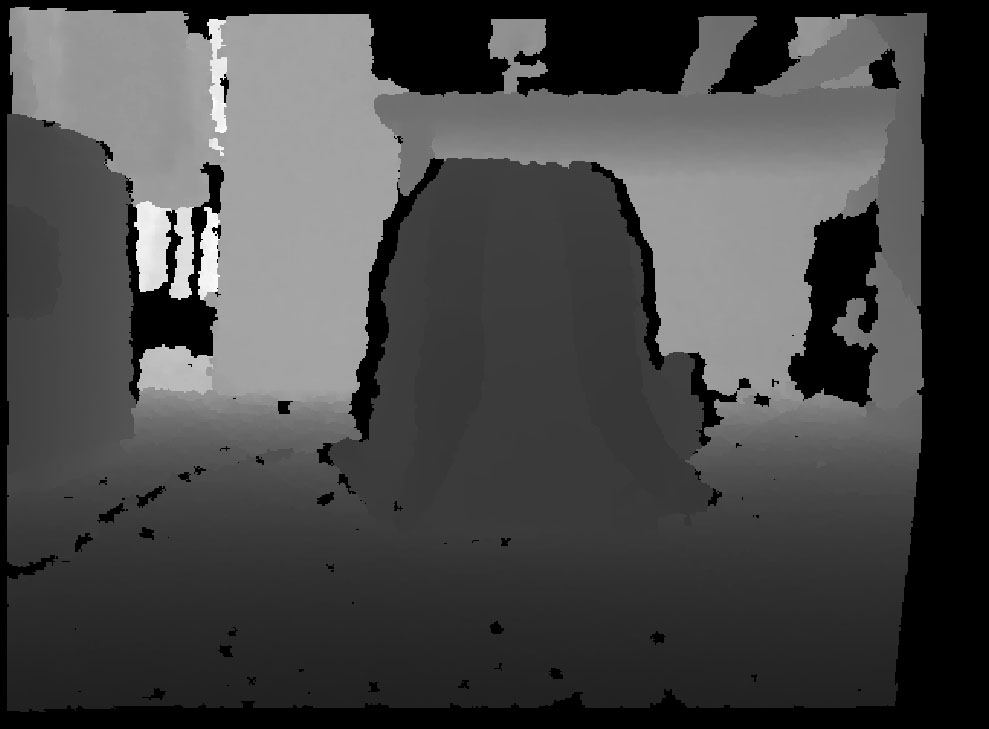
\includegraphics[width=8cm]{eval_rgbd1.jpg}
	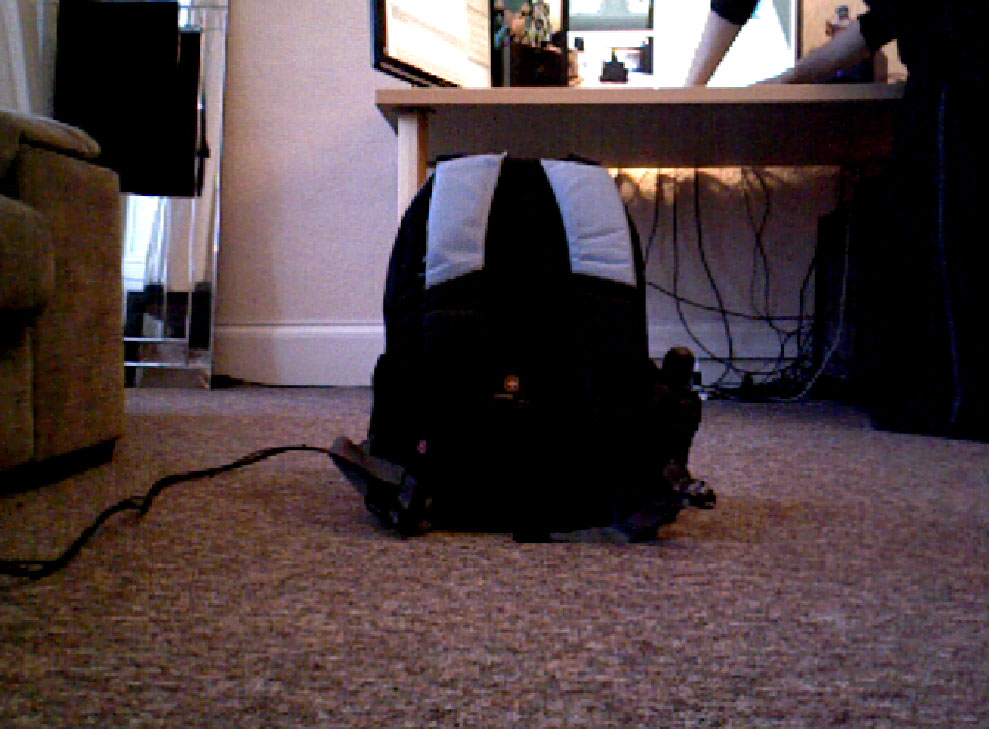
\includegraphics[width=8cm]{eval_rgbd2.jpg}
	\caption{A display of the generated map after an obstacle has been placed in front of the robot---a backpack in this case---along with the direct RGB (bottom left) and depth (bottom right) outputs from the RGB-D camera. The resulting blocks from the bag can be seen on the map. Notably, the bag appears as a rather patchy grouping of blocks but would still be enough to trigger any avoidance routines from the navigation system.}
	\label{fig:eval_map_bag}
\end{figure}

The resulting output after having placed the obstacle in front of the robot can be seen in \autoref{fig:eval_map_bag}. In this case, the surrounding environment was mapped quite accurately once again. The bag was also detected and mapped, however the resulting points were rather disjointed. The full shape of the obstacle was not mapped completely, even though it can be seen quite clearly in the raw imagery. Even though this was the case, the navigational system would have still been able to route around these points as the base footprint of the object can still be seen.

\subsubsection{Mapping During Walk Cycle}

The final experiment aimed to test the accuracy of the mapping component as the robot moved around the environment using the tripod gait. In particular, the robot would walk around the environment along the path as shown on \autoref{fig:eval_plan}, starting from the start position and ending at the end position. Manual control through the gamepad controller would be used for this test, rather than relying on the navigational system. The same \emph{rviz} configuration from previous tests would be used to visually observe the generated map for accuracy.

\begin{figure}[h]
	\centering
	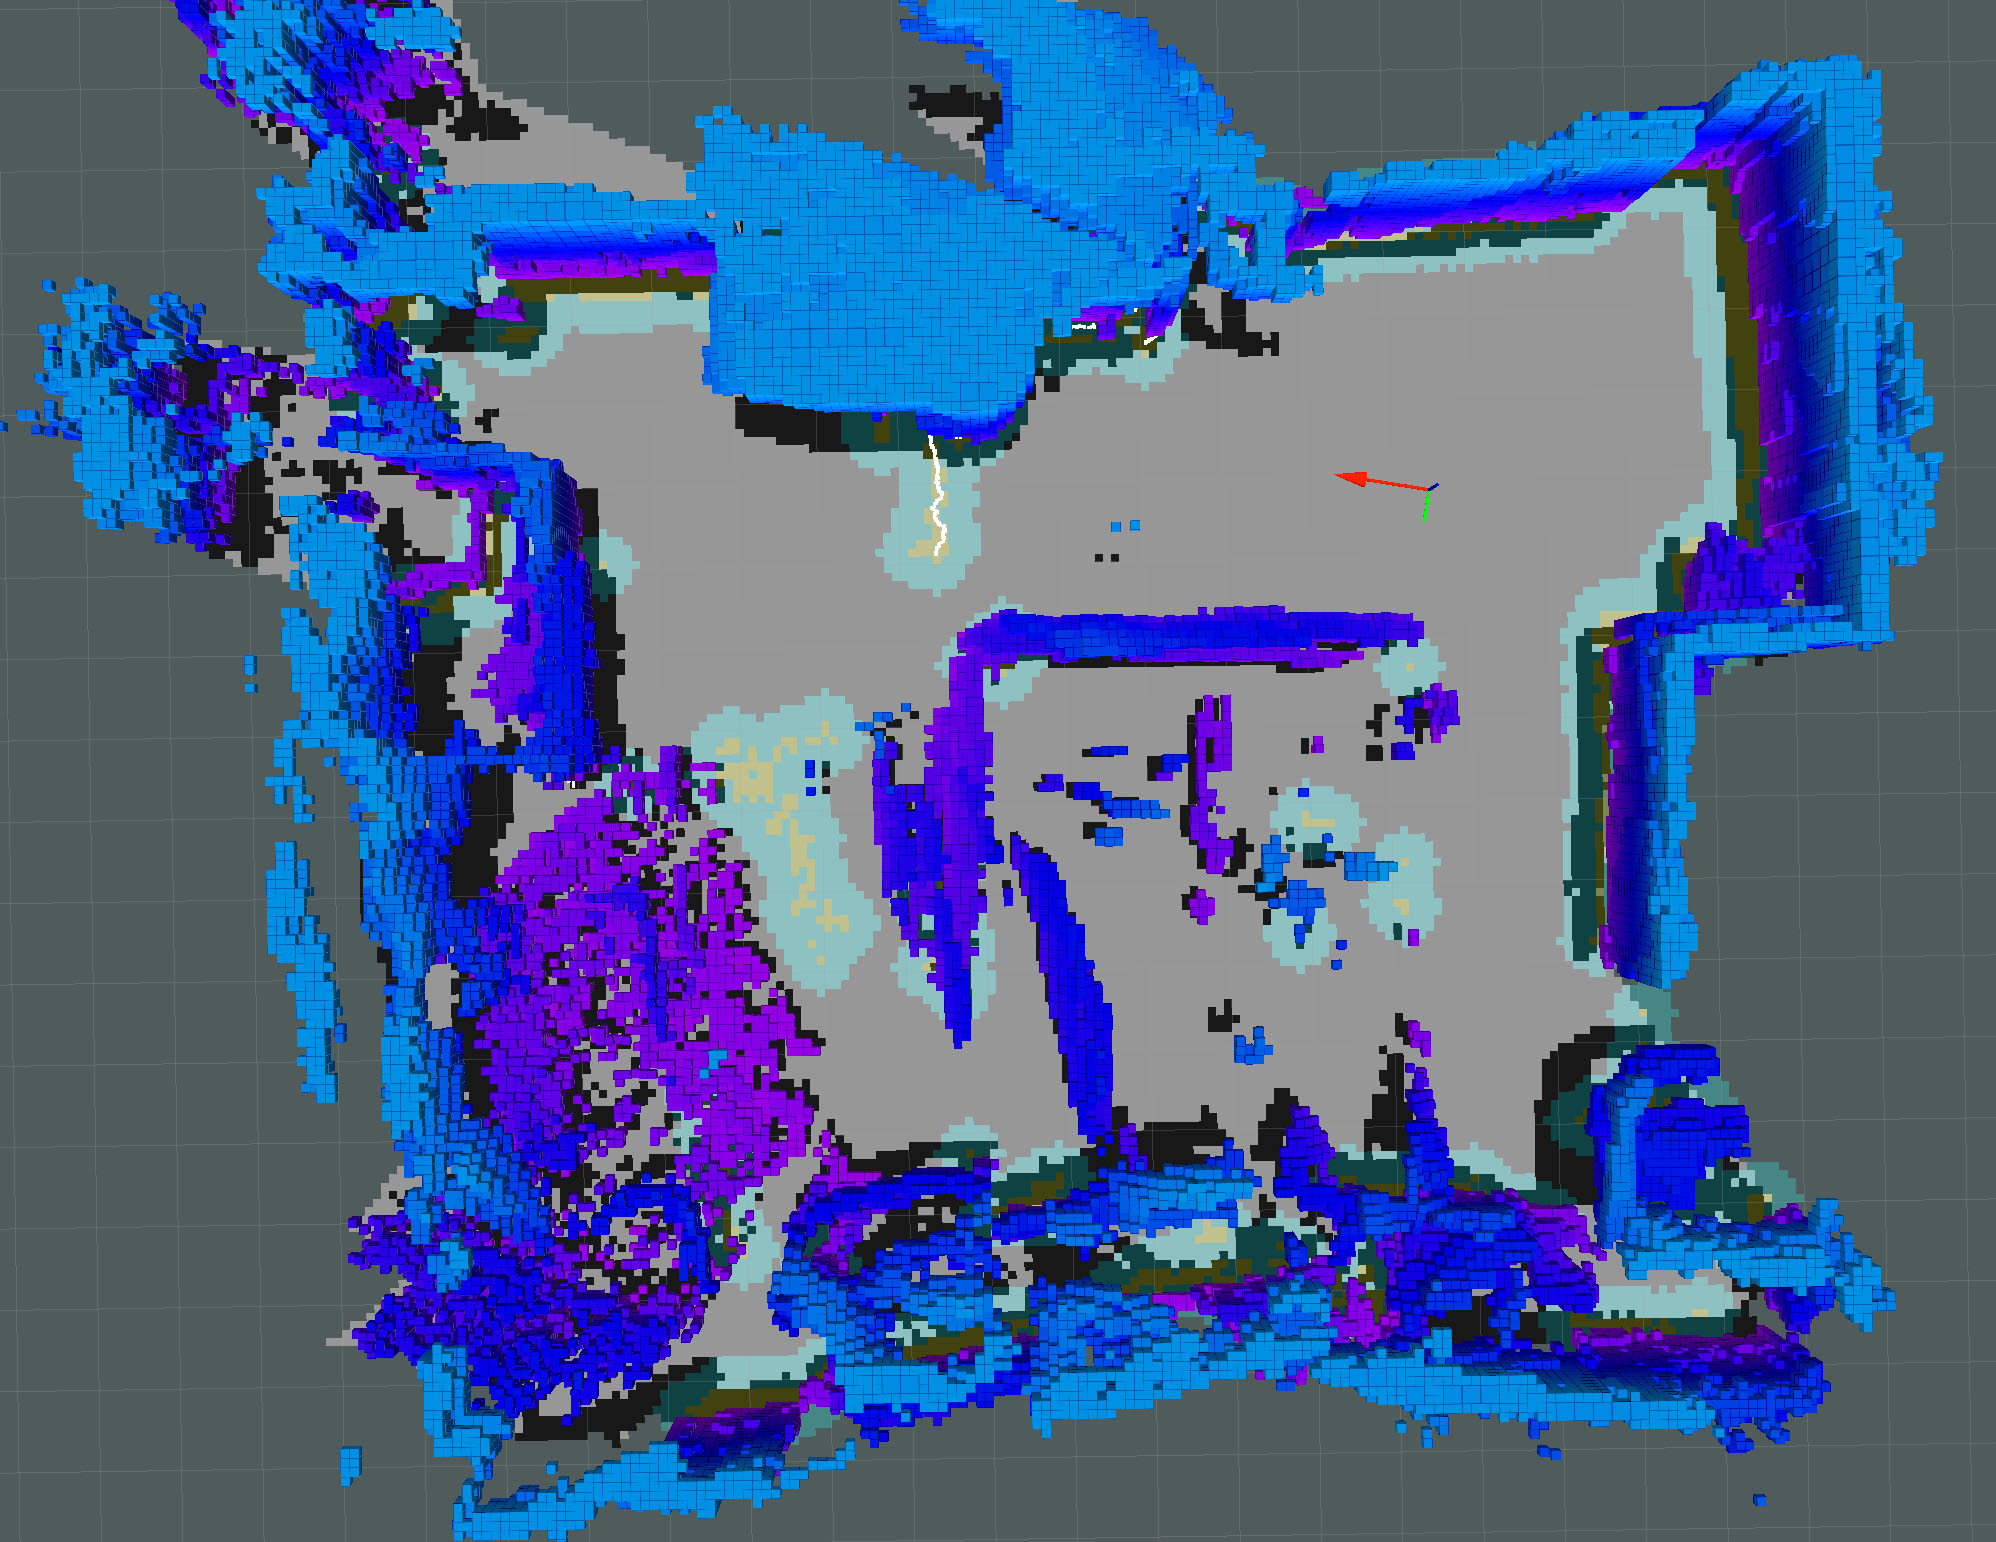
\includegraphics[width=16cm]{eval_map3.jpg}
	\caption{A display of the generated map after the robot has had a tour around the environment, as provided by RViz. It can be seen that the mapping system correctly generated a reasonable facsimile of the surrounding environment, however there is a large amount of distortion due to the drift from the visual locomotory system. Additionally, a rather large patch of the floor (bottom left, specifically) has been detected as an obstacle. As an aside, a strange effect results from the mirror that sits in the corner of the environment (top left, specifically).}
	\label{fig:eval_map_room}
\end{figure}

The resulting map output for this test is shown in \autoref{fig:eval_map_room}. While the mapping component generated a reasonable facsimile of the surrounding environment, there were significant distortions due to the positional drift caused by the visual odometery system, particularly when the robot was rotating. Specifically, the detected walls of the environment should have been at right angles to each other but are shown to be somewhat askew. As the mapping component depends entirely on the visual odometry component for a positional fix, there is little that could have been done to solve this issue. An additional facility to localise the robot's position based on the map rather than relative motion may have been helpful in this case, as it would be able to correct for any drift.

\section{Navigation}

To test the navigation subsystem, the following set of experiments were performed. In particular, we looked to test the time taken and accuracy for the movements generated by this system when asked to reach a particular goal. To give a comparison, we would compare the results to that of those given from manual movements following an ``ideal'' path. This would require full integration and correct operations of all previously tested subsystems thus far, as the navigation subsystem relies on all of these subsystems for its own operation. 

Specifically, two different sets of experiments were performed. One set would test autonomous navigation on a direct path with minimal rotation whereas the other would test a more complex path involving multiple turns.

\subsection{Direct Path}

The first set of experiments aimed to test the navigation system given a goal directly in front of the robots, such that no rotations were required. The target goal would be $3$m forward from the robot's starting position. At the start of each test, the control system would be reset. Once the system was ready, a goal would be set $3$m from the starting position with a forward heading using the target tool on \emph{rviz}. Time would be recorded and general accuracy observed. As a comparison, the time taken to move along the path manually using the gamepad controller would be recorded. 

Dynamic obstacle avoidance would also be tested. An object---in this case a backpack as used in the previous examples---would be placed in front of the robot as it reached $1$m. How well the navigation system managed to move around this object would then be observed.

\subsubsection{Without Obstacle}

The first experiment in this set would evaluate accuracy and timing without any obstacles in the path of the robot. First, a number of manual movements were done as a control which gave a resulting average time of $36.164$s from start point to end point. Following this, tests using the navigation system were performed. These tests gave a resulting average time of $45.495$s from start point to end point, giving an average increase in time of $9.331$s. A full listing of results can be seen in \autoref{tab:eval_nav_dp_wo}.

The navigation subsystem spends a lot of time trying to keep the robot directly on its planned path---as one would expect---but this resulted in a number of unnecessary rotations, slowing down the overall movement. Additionally, some amount of processing time is needed for the system to compute a path. These are the most likely sources of this time increase. In general, however, the motions given by the system were reasonably accurate.

\subsubsection{With Obstacle}

The second experiment in this set would evaluate the accuracy and timing of the navigational system, but this time after an obstacle had been placed in front of the robot while it was walking. As before, a number of manual movements were performed for control---assuming that an ideal path was to curve around the obstacle. The manual movements gave an average time of $51.136$s. Following this, tests using the navigation system alone were performed. These autonomous tests gave a resulting average time of $1$m $5.677$s from start point to end point, giving an average increase in time of $14.541$s. A full listing of results can be seen in \autoref{tab:eval_nav_dp}.

\begin{figure}[h]
	\centering
	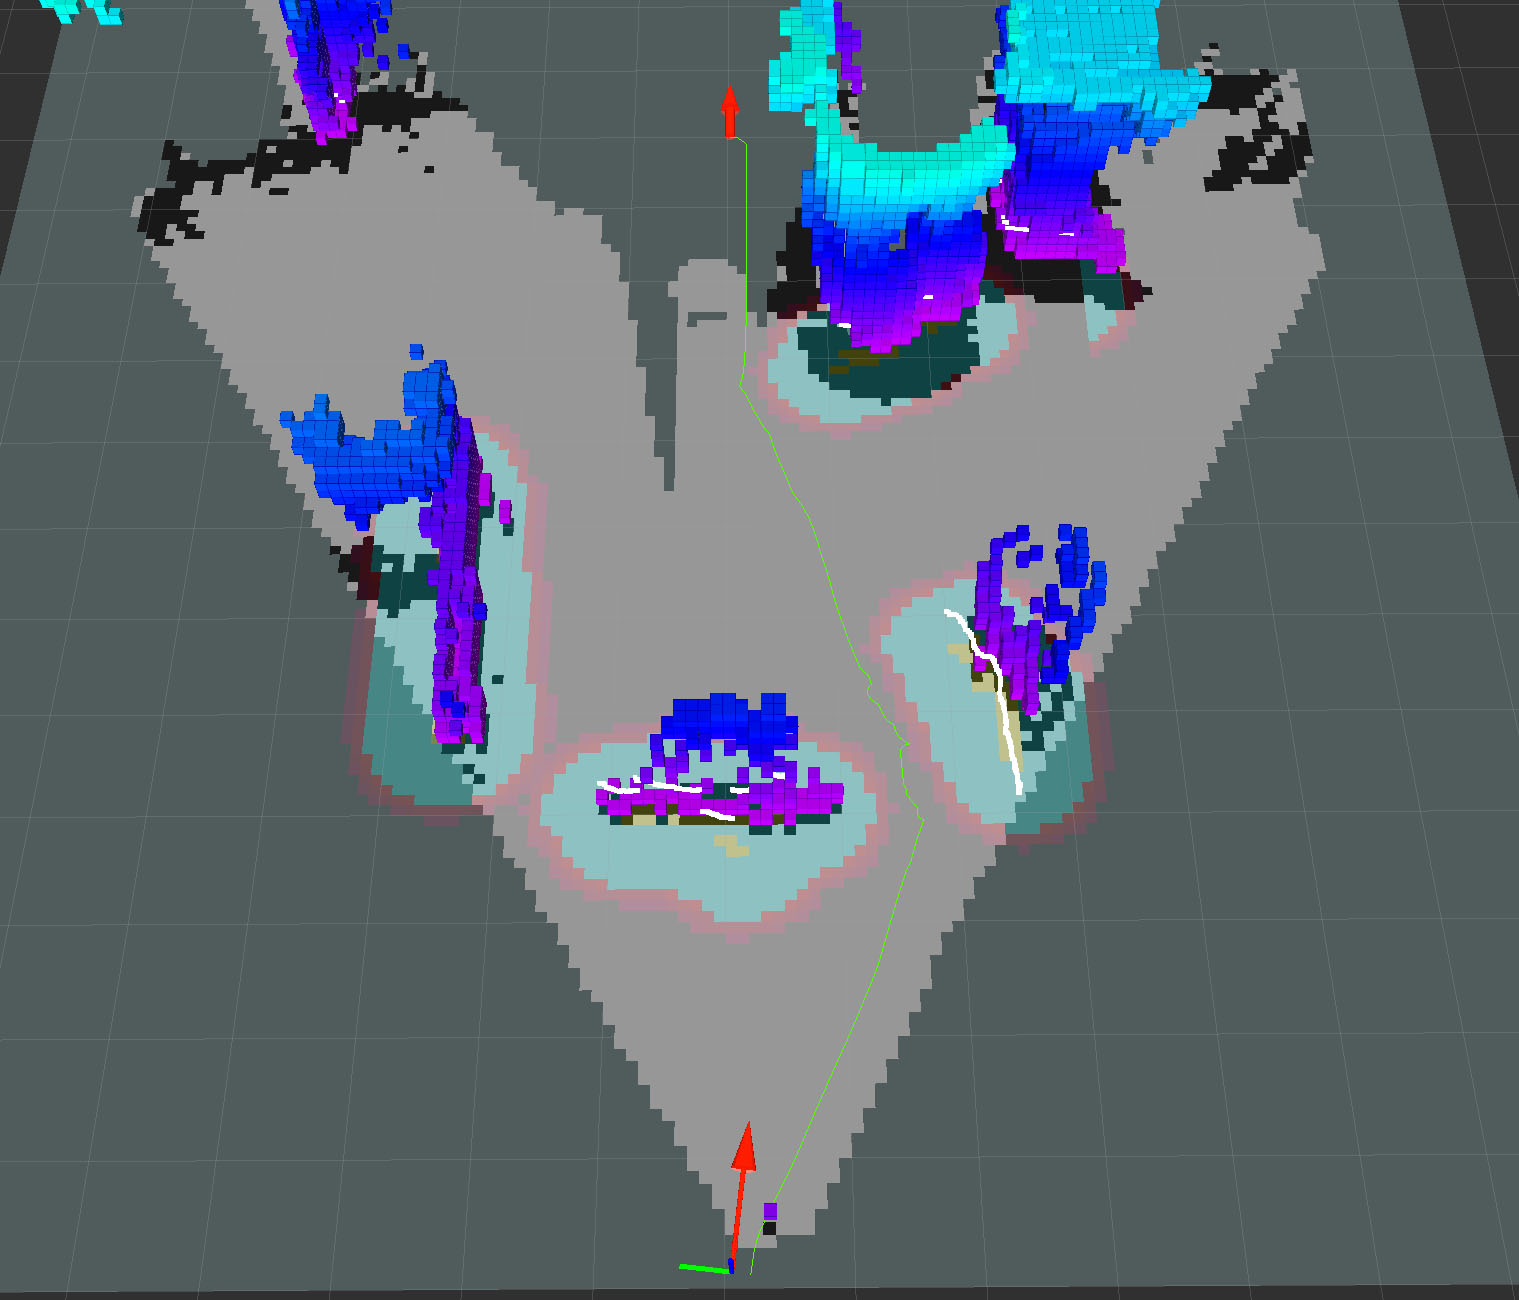
\includegraphics[width=14cm]{eval_nav.jpg}
	\caption{A display of the planned path from the autonomous navigation system after an obstacle---in this case a backpack as before---has been placed in front of the robot. Prior to this image the planned path was directly ahead with no rotations. However, after the obstacle has been placed in front of the robot, the navigation system automatically recalculates the path such that it avoid the obstacles. The circular patterns on the ground plane indicate obstacle radii on the planner's avoidance costmap.}
	\label{fig:eval_nav}
\end{figure}

An example of the path generated after the bag has been placed in front of the robot can be seen in \autoref{fig:eval_nav}. The causes of this time increase were similar to those mentioned in the previous test, but with the added rotational visual odometry drift. This rotational drift from the causes the navigation system to try and correct itself unnecessarily even though it is already in the correct position. Regardless, the robot was able to navigate around the bag successfully each time.

\subsection{Complex Path}

The second set of experiments aimed to test the navigation subsystem given a goal that would create a complex path. In these cases, the starting position and target end position would be those shown in \autoref{fig:eval_map_room}. This would show that the robot was capable of moving from one side of the room to the other. Two experiments would be performed: one where the robot had a chance to move around before hand such that the environment was already mapped, and the other where the control system had no knowledge of the environment before hand. As before, time would be recorded and general accuracy observed. A manually controlled walk would be done for time comparison.

\subsubsection{Known Environment}

The first experiment in this set would aim to prove the accuracy and efficiency of the navigation subsystem in a known environment. A number of manual tours around the ``ideal'' path would be performed before hand to get a control on timing as well as to provide a good mapping of the environment. After this, the robot would be placed at its starting position and commanded to navigate to the end position, as shown on \autoref{fig:eval_map_room}.

The manual movements from this experiment gave an average time of $2$m $5.649$s. For the autonomous navigation tests, the resulting average time was $2$m $30.561$s giving a difference of $24.912$s. This additional time is for the same reasons as explained in the previous tests. In one case, the test did not finish due to a cascading set of failures. Specifically, the navigation subsystem managed to propel the robot into a nearby obstacle whereupon the visual odometry system ceased to give a positional fix. This required a full restart of the control system and, thus, was counted as a ``did not finish'' result.

Generally, however, the test was successful. The visual odometry drift issue was still apparent overall but not enough to cause any significant problems.

\subsubsection{Unknown Environment}

The final experiment would aim to prove the accuracy and efficiency of the navigation system in an unknown environment. Unlike the previous test, no manual walking was performed to provide any mapping information. The control system would be started cleanly and then be expected to navigate from one side of the environment to the other. Manual timing information from the previous experiment would be used as a control---it did not make much sense for us to run the tests again when we ourselves already knew the environment. The navigation subsystem would have to detect and avoid obstacles to get to the end position as it moved the robot around. 

Results from this test were varied. Out of the seven tests that completed successfully, the average time taken was $3$m $37.486$s giving a time difference from the control of $1$m $31.837$s. For those tests that did not complete successfully, similar issues as of those in the previous experiment occurred. Upon receiving the target goal, the navigation system immediately assumes it can get there directly as it has no information telling it otherwise. In these failure cases, the robot would get stuck facing the obstacle as the visual odometry system fails to detect any features from it due to being too close, causing a cascading failure of the mapping and navigational systems. In most cases, however, the robot was able to detect and adjust its path accordingly before it could get stuck. 

Further tweaking of both the navigation and visual odometry systems is needed to improve upon these results.
\chapter{Conclusion}
\label{chap:conclusion}

%%%%%%%%%%%%%%%%%%%%%%%%%%%%%%%%%%%%%%%%%%%%%%%%%%%%%%%%%%%%%%%%%%%%%%%%%%%%%%%%%%%%%%%%%%%%%%%%%%%%

\section{Summary}
Robots are awesome, man.

%%%%%%%%%%%%%%%%%%%%%%%%%%%%%%%%%%%%%%%%%%%%%%%%%%%%%%%%%%%%%%%%%%%%%%%%%%%%%%%%%%%%%%%%%%%%%%%%%%%%

\section{Further Work}

This final section will detail a number of ways in which the project could be developed further. Much of this additional functionality could be provided by existing standard or community-provided ROS packages, however further research is necessary to prove the adequacy of such packages. Furthermore, some of these suggestions require additional or even entirely new hardware. These would require new drivers, control software, not to mention the hardware integration itself.

\subsection{Improved Hardware}
The servos currently in use in the robot are extremely cheap, fast and have incredible amounts of torque. Unfortunately, this comes at the cost of accuracy and build quality. Generally, the robot requires complete calibration every time it is powered on to ensure correct operation.

\subsection{Untethered \& Cloud Operation}
The robot is only capable of tethered operation in its current hardware configuration. Specifically, a large bundle of cables protrudes from the back of the robot, connecting the RGB-D camera and servo controller to a nearby computer and power source. This restricts the robot to 5 meter radius around the equipment, as USB devices tend to stop functioning correctly with cables above this length without active boosters. 

The decision to limit to tethered operation only was to, primarily, reduce the complexity of the robot hardware itself while the control system was being developed. Batteries require additional circuitry, such as voltage converters and charging circuits. Furthermore, the power requirements for the robot are quite high posing somewhat of a potential health risk, as the robot draws 10A at 6V at full operational speed. Now that a working control system is implemented, these issues are no longer a concern.

Furthermore, the sensing system requires a particularly high performance machine to achieve good results. Even if it were possible to interface with the RGB-D sensor through a microcontroller, it would in no shape or form be able to meet these performance demands.

However, it would be possible to exploit the distributed nature of ROS to alleviate these issues. A Beaglebone Black, for example, could be attached to the robot. This could connect directly to the RGB-D camera and servo controller over USB as the current system does. Subsystems that interface with the hardware would run on this embedded system. Another machine could then be dedicated to performing the complex processing tasks.

This idea could be expanded to make use of cloud services such as Amazon EC2 and Microsoft Azure. Rather than running the performance demanding nodes on a physical machine, they could be ran on a number of virtual machines. 

\subsection{Inverse Kinematics}
More accurate walk cycle. Advanced movement, tilting. Sweeping.

\subsection{Further Sensor Hardware \& Environment Interpretation}
Accelerometers for automatic calibration, odometery. Distance sensors as insect-like feelers. Use of microphones on Xtion.  

\subsection{Facial Recognition}
ROS already has packages for this. More complex behaviour in general.
\begin{appendices}

\chapter{Demonstration Video}

A demonstration video of the robot can be found at \url{http://youtu.be/efLMad5wh7w}.

\chapter{Source Code}

A repository containing the source code of the implemented robot control system can be found on GitHub at \url{https://github.com/Knifa/HexapodKit}.

\chapter{Evaluation Results}

This appendices show the full results from the control system evaluation.

\section{Visual Odometery}

These tables contain the resulting $(x, y)$ position and $\theta_z$ angle reported by the visual odometery system after various movements. The positions are relative to the robot's starting position---i.e., the starting position is $(0, 0)$.

\subsection{Linear Motion}

\begin{table}[!h]
	\centering
	\begin{tabular}{ r r r }
		\toprule
		\multicolumn{3}{c}{\textbf{Manual}} \\
		\midrule
		\textbf{$x$} & \textbf{$y$} & \textbf{$\theta_z$} \\
		\midrule
		$0.905$m &
		$0.048$m &
		$3.565$\textdegree{} \\

		$0.906$m &
		$0.007$m &
		$-0.709$\textdegree{} \\

		$0.932$m &
		$0.024$m &
		$3.648$\textdegree{} \\

		$0.932$m &
		$-0.007$m &
		$2.786$\textdegree{} \\

		$0.928$m &
		$-0.006$m &
		$-3.599$\textdegree{} \\

		$0.938$m &
		$-0.010$m &
		$-2.813$\textdegree{} \\

		$0.928$m &
		$0.028$m &
		$2.752$\textdegree{} \\

		$0.932$m &
		$-0.020$m &
		$-3.681$\textdegree{} \\

		$0.934$m &
		$-0.028$m &
		$0.782$\textdegree{} \\

		$0.909$m &
		$0.005$m &
		$1.981$\textdegree{} \\

		\midrule
		$0.924$m &
		$0.004$m &
		$0.471$\textdegree{} \\
		\bottomrule
	\end{tabular}
	\hspace{2ex}
	\begin{tabular}{ r r r }
		\toprule
		\multicolumn{3}{c}{\textbf{Walking}} \\
		\midrule
		\textbf{$x$} & \textbf{$y$} & \textbf{$\theta_z$} \\
		\midrule
		$0.936$m &
		$-0.019$m &
		$-0.871$\textdegree{} \\

		$0.949$m &
		$0.046$m &
		$-6.362$\textdegree{} \\

		$0.944$m &
		$0.039$m &
		$1.971$\textdegree{} \\

		$0.955$m &
		$-0.046$m &
		$5.363$\textdegree{} \\

		$0.968$m &
		$0.057$m &
		$-3.224$\textdegree{} \\

		$0.934$m &
		$0.021$m &
		$-0.548$\textdegree{} \\

		$0.949$m &
		$0.037$m &
		$-0.27$\textdegree{} \\

		$0.987$m &
		$-0.044$m &
		$-2.067$\textdegree{} \\

		$0.968$m &
		$0.039$m &
		$1.594$\textdegree{} \\

		$0.934$m &
		$0.001$m &
		$6.325$\textdegree{} \\

		\midrule
		$0.952$m &
		$0.013$m &
		$0.191$\textdegree{} \\
		\bottomrule
	\end{tabular}

	\caption{Results from the visual odometry system after having moved the robot by $1$m both by hand and using the walk cycle.}
	\label{tab:eval_vo}
\end{table}

\subsection{Angular Rotation}

\begin{table}[!h]
	\centering
	\begin{tabular}{ r r r }
		\toprule
		\multicolumn{3}{c}{\textbf{Manual}} \\
		\midrule
		\textbf{$x$} & \textbf{$y$} & \textbf{$\theta_z$} \\
		\midrule
		$0.066$m &
		$-0.027$m &
		$90.023$\textdegree{} \\

		$0.088$m &
		$-0.059$m &
		$88.592$\textdegree{} \\

		$0.199$m &
		$0.029$m &
		$90.419$\textdegree{} \\

		$0.097$m &
		$0.069$m &
		$88.109$\textdegree{} \\

		$0.055$m &
		$-0.039$m &
		$88.51$\textdegree{} \\

		$0.176$m &
		$0.074$m &
		$88.438$\textdegree{} \\

		$0.055$m &
		$-0.005$m &
		$91.587$\textdegree{} \\

		$0.14$m &
		$0.056$m &
		$89.128$\textdegree{} \\

		$0.055$m &
		$0.004$m &
		$88.484$\textdegree{} \\

		$0.064$m &
		$-0.058$m &
		$89.676$\textdegree{} \\

		\midrule
		$0.1$m &
		$0.004$m &
		$89.296$\textdegree{} \\
		\bottomrule
	\end{tabular}
	\hspace{2ex}
	\begin{tabular}{ r r r }
		\toprule
		\multicolumn{3}{c}{\textbf{Walking}} \\
		\midrule
		\textbf{$x$} & \textbf{$y$} & \textbf{$\theta_z$} \\
		\midrule
		$0.152$m &
		$0.068$m &
		$88.937$\textdegree{} \\

		$0.283$m &
		$-0.011$m &
		$89.188$\textdegree{} \\

		$0.197$m &
		$-0.046$m &
		$92.523$\textdegree{} \\

		$0.14$m &
		$-0.044$m &
		$85.965$\textdegree{} \\

		$0.119$m &
		$0.01$m &
		$86.522$\textdegree{} \\

		$0.098$m &
		$-0.072$m &
		$85.157$\textdegree{} \\

		$0.239$m &
		$0.021$m &
		$93.074$\textdegree{} \\

		$0.122$m &
		$0.015$m &
		$92.791$\textdegree{} \\

		$0.169$m &
		$-0.044$m &
		$90.951$\textdegree{} \\

		$0.199$m &
		$-0.077$m &
		$87.728$\textdegree{} \\

		\midrule
		$0.172$m &
		$-0.018$m &
		$89.284$\textdegree{} \\
		\bottomrule
	\end{tabular}

	\caption{Results from the visual odometry system after having rotated the robot by $90$\textdegree{} both by hand and using the walk cycle.}
	\label{tab:eval_vo_rot}
\end{table}

\section{Navigation}

\subsection{Direct Path}

\subsubsection{Without Obstacle}

\begin{table}[!h]
	\centering
	\begin{tabular}{ c }
		\toprule
		\textbf{Manual} \\
		\midrule
		Time \\
		\midrule
		$34.203$s \\

		$34.411$s \\

		$37.379$s \\

		$34.983$s \\

		$38.032$s \\

		$34.401$s \\

		$34.988$s \\

		$38.167$s \\

		$36.907$s \\

		$38.166$s \\

		\midrule
		$36.164$s \\
		\bottomrule
	\end{tabular}
	\hspace{2ex}
	\begin{tabular}{ c }
		\toprule
		\textbf{Autonomous} \\
		\midrule
		Time \\
		\midrule
		$51.267$s \\

		$45.533$s \\

		$40.938$s \\

		$46.094$s \\

		$42.858$s \\

		$48.690$s \\

		$44.141$s \\

		$45.372$s \\

		$44.847$s \\

		$45.208$s \\

		\midrule
		$45.495$s \\
		\bottomrule
	\end{tabular}
	\caption{Time taken for the robot to autonomously navigate a direct $3$m path.}
	\label{tab:eval_nav_dp_wo}
\end{table}

\subsubsection{With Obstacle}

\begin{table}[!h]
	\centering
	\begin{tabular}{ c }
		\toprule
		\textbf{Manual} \\
		\midrule
		Time \\
		\midrule
		$0$m $50.406$s \\

		$0$m $50.183$s \\

		$0$m $50.782$s \\

		$0$m $51.81$s \\

		$0$m $51.012$s \\

		$0$m $50.406$s \\

		$0$m $52.334$s \\

		$0$m $52.264$s \\

		$0$m $51.475$s \\

		$0$m $50.684$s \\

		\midrule
		$0$m $51.136$s \\
		\bottomrule
	\end{tabular}
	\hspace{2ex}
	\begin{tabular}{ c }
		\toprule
		\textbf{Autonomous} \\
		\midrule
		Time \\
		\midrule
		$1$m $4.771$s \\

		$1$m $8.007$s \\

		$1$m $4.724$s \\

		$1$m $0.816$s \\

		$1$m $7.04$s \\

		$1$m $6.758$s \\

		$1$m $1.963$s \\

		$1$m $8.458$s \\

		$1$m $5.232$s \\

		$1$m $9.0$s \\

		\midrule
		$1$m $5.677$s \\
		\bottomrule
	\end{tabular}
	\caption{Time taken for the robot to autonomously navigate a direct $3$m path after an obstacle has been placed $1$m from the starting position.}
	\label{tab:eval_nav_dp}
\end{table}

\subsection{Complex Path}

\subsubsection{Known Environment}

\begin{table}[!h]
	\centering
	\begin{tabular}{ c }
		\toprule
		\textbf{Manual} \\
		\midrule
		Time \\
		\midrule
		$2$m $5.643$s \\

		$2$m $10.224$s \\

		$2$m $7.821$s \\

		$2$m $8.206$s \\

		$2$m $4.561$s \\

		$2$m $1.542$s \\

		$2$m $2.964$s \\

		$2$m $2.178$s \\

		$2$m $9.315$s \\

		$2$m $4.037$s \\

		\midrule
		$2$m $5.649$s \\
		\bottomrule
	\end{tabular}
	\hspace{2ex}
	\begin{tabular}{ c }
		\toprule
		\textbf{Autonomous} \\
		\midrule
		Time \\
		\midrule
		$2$m $29.284$s \\

		DNF \\
				
		$2$m $28.418$s \\

		$2$m $34.716$s \\

		$2$m $34.484$s \\

		$2$m $25.634$s \\

		$2$m $26.558$s \\

		$2$m $32.505$s \\

		$2$m $29.575$s \\

		$2$m $33.873$s \\

		\midrule
		$2$m $30.561$s \\
		\bottomrule
	\end{tabular}
	\caption{Time taken for the robot to navigate a known environment, specifically the path shown in \autoref{fig:eval_plan}. Average time taken in this case did not include \emph{DNF} results.}
	\label{tab:eval_nav_cp_known}
\end{table}

\subsubsection{Unknown Environment}

\begin{table}[!h]
	\centering
	\begin{tabular}{ c }
		\toprule
		\textbf{Autonomous} \\
		\midrule
		Time \\
		\midrule
		$3$m $47.259$s \\

		$3$m $46.573$s \\

		$3$m $24.283$s \\

		DNF \\

		DNF \\

		$3$m $23.027$s \\

		$3$m $41.999$s \\

		$3$m $32.822$s \\

		$3$m $46.440$s \\

		DNF \\

		\midrule
		$3$m $37.486$s \\
		\bottomrule
	\end{tabular}
	\caption{Time taken for the robot to navigate an unknown environment, specifically the path shown in \autoref{fig:eval_plan}. Average time taken in this case did not include \emph{DNF} results.}
	\label{tab:eval_nav_cp_unknown}
\end{table}

\end{appendices}

%%%%%%%%%%%%%%%%%%%%%%%%%%%%%%%%%%%%%%%%%%%%%%%%%%%%%%%%%%%%%%%%%%%%%%%%%%%%%%%%%%%%%%%%%%%%%%%%%%%%

\renewcommand{\bibname}{References}
\bibliographystyle{plain}
\bibliography{report}

\end{document}
